\section{Planned Experiments and Pre-registered Criteria}
\label{sec:plan}

이 절의 표는 모두 결과 예정 칸(\todoexp)이며, 판정 기준은 실행 전에 고정한다. 각 표의 캡션에 우리가 기대하는 결과와, 그 결과가 지지하거나 반박하는 주장을 한 문장씩 적는다. 기대와 다른 결과가 나와도 같은 표에 그대로 보고한다. 실험은 세 줄기로 나뉜다(\cref{tab:roadmap}). 아래층 확정 규칙 줄기는 E0(지연·결정성) $\rightarrow$ E0.5(오프라인 표 재생) $\rightarrow$ E1(보정) $\rightarrow$ E-M4다. 아래층 입력·학습 줄기는 공개 실물 데이터와 시뮬 데이터에서 E-TC와 그 확인, E-CAM3, E-MA1b, E-MA2, E-MA3를 돈다. Astra 줄기는 E-Astra-motion 탐침 $\rightarrow$ E-SR0 $\rightarrow$ 조건 강화(E-SR1b, E-SR1c, 실데이터 E-SR1d) $\rightarrow$ Astra 한 호출 정확도(프롬프트 검진, E-ACC)와 Astra에 최적인 단독 팔(E-Astra-solo) $\rightarrow$ VLA 단독 폐루프 온전성 관문 $\rightarrow$ E-Couple $\rightarrow$ E-Astra-necessity다. VLA는 Astra의 구간 계획과 교정이 옳다는 전제로 움직이므로, Astra의 호출 단위 정확도를 먼저 최대화한다(정본 §94). 추가 학습(E-AT, E-MAR-real)은 실데이터에서만 한다(정본 §89). 장기 목표는 Astra를 학습 가능한 크기의 LLM으로 대체하는 것이며(E-TEACH, 정본 §96), 상위 모델에 주는 맥락은 로봇과 인식에서 자동으로 만든다(정본 §97). 정본 §92의 파이프라인 배치는 확정했지만, 그 배치가 기대는 전제 12개(P1--P12)와 가설 H-L(P13)은 아직 검증 중이다(\cref{tab:premises}). 세 줄기가 모인 뒤 본 평가(RD)를 한다. 유료 실험은 사전 등록에 ``이 결과로 바꾸는 설계 결정''과 ``이 표본으로 그 결정을 가를 수 있는가''를 먼저 적고, 무료 로컬 모델로 파이프라인을 먼저 돌린 뒤, 단계 관문마다 결함이 보이면 멈추고 다시 설계하는 자체 검사를 거친다. 과금되는 호출은 목적·호출 수·예상 비용을 먼저 제안하고 사용자의 명시적 허락을 받은 뒤에만 실행한다. 이 규칙은 실제 Astra 클라이언트를 쓰는 모든 경로의 유료 실행 가드로 코드에도 걸려 있다. 상위 모델 줄기는 E-TEACH-L8 $\rightarrow$ 출력 형식(E-PT, ND) $\rightarrow$ 데이터 형태와 비율(E-XEMB8) $\rightarrow$ 35B 순이다(\cref{sec:plan_pt,sec:plan_data}). 공개 실물 데이터의 소규모 학습 시험(S-E2E, 규모 곡선, E-TC와 그 확인, E-CAM3, E-MA1b)은 수치 앞에 모두 파이프라인 시험임을 밝히며, 입력 형식과 학습 보강을 고르는 데에만 쓴다.

\begin{table}[t]
\centering
\scriptsize
\setlength{\tabcolsep}{2.5pt}
\begin{tabular}{@{}p{0.20\linewidth}p{0.46\linewidth}p{0.26\linewidth}@{}}
\toprule
실험 & 가르는 결정 & 상태 \\
\midrule
E-TC, 확인 & 결정 입력에 움직임 줄·과거 프레임 & 움직임 줄 채택·확인 \\
E-MA1 / E-MA1b & 미래 궤적 보조 손실 & G0 실패; 3D판 불채택(\tentative{+0.0031}); 이미지판 \tentative{예정}(R2) \\
E-CAM3 & VLA 입력 카메라 2대 대 3대 & 불채택(\tentative{+0.0014}, p95 \tentative{+11.7\%}) $\rightarrow$ 2대 유지 \\
E-MA2 & VLA가 Astra 명령을 보는가(문장·화살표) & NONE: 결정층만 명령을 따름 $\rightarrow$ 코드 편향만 \\
E-MA3 & expert 층별 KV 조건 & 불채택(청크 오차 \tentative{$-$2.19\%} $<$ 문턱 5\%) \\
E-Astra-motion & 요청 형식 F0/F1, 카메라 구성, 실제 비용·지연 & 완료: F0, 나이 상한 15\,s, 파지 확정 T1·V1h \\
E-SR0 & 연속 행동이 조이스틱을 따르는가 & WEAK(\tentative{0.340}, \tentative{0.431}; 우연 0.33) $\rightarrow$ 청크·손끝 기준 \\
E-SR1b & 결정 드롭아웃·CFG·되짚기 라벨로 준수 0.8 & NOT\_REACHED(최고 \tentative{0.598}) \\
E-SR1c & 먼 구간 반사실 분기(R2 시뮬) & ADOPT\_C1(먼 구간 \tentative{0.991}) \\
E-SR1d & 같은 분기를 실데이터에(P1) & NOT\_REACHED(\tentative{0.339$\rightarrow$0.536}) $\rightarrow$ 청크·손끝 경유 유지 \\
E-NOV0 & 백본 특징 새로움으로 호출 거르기 & NONE(\tentative{0.570}); 확신도 \tentative{0.804}는 판정 밖 \\
E-SR1e & 실데이터 분기 레시피(학습 길이·분기 비율, 대조 안내) & 과소적합 진단 뒤 사전 등록, \tentative{진행 중} \\
E-CONF & 결정 확신도 운용(§95)을 새 표본에서 & NONE(실데이터 \tentative{0.748} $<$ 0.75) $\rightarrow$ 기록만 \\
프롬프트 검진, E-ACC & Astra 한 호출 명령 정확도(P4, §94) & v2 채택; 7--10\,cm 목표 어긋남 알아채기 \tentative{0/13} \\
E-Astra-solo & Astra에 최적인 단독 팔(§93) & \tentative{7/7}(파일럿 4 + 전체 3), 단계 재설계로 \tentative{진행 중} \\
E-Couple 사전 실행 & 결합 배관(무료, 판정 없음) & 배관 통과; VLA 단독 \tentative{0/12} $\rightarrow$ 관문 추가 \\
E-VLA-solo & VLA 단독의 의미, 재생 속도 낮추기 & 모든 조건 \tentative{0/12}(규칙 기준선 \tentative{12/12}); 속도 낮추기 불채택, 멈춤 고리 확인 \\
E-MAR-real & 실데이터 포인팅 궤적 보조(§89) & 불채택(\tentative{+0.0047}) \\
E-OpenVLM-proxy & 오픈 VLM급 모델이 영샷으로 Astra 자리를 맡는가 & gpt-5.2 대리 \tentative{0/4}(인식) \\
E-TEACH & 학습 가능한 크기 LLM으로 Astra 대체(§96) & L8(8B, 참값 라벨) DEV \tentative{4/4}, 영샷 \tentative{0/4}; 다양화·OOD \tentative{예정} \\
자동 맥락 A0--A2 & 로봇 자기 정보 자동 생성·장면 인식 자동화(§97) & 설계 끝, \tentative{예정} \\
E-PT / ND & 상위 출력 형식: 점 찍고 행동, 깊이 없이 모델이 거리를 앎(§97 보충 2) & 사전 등록(무료), 주 팔 ND-1·ND-2, \tentative{진행 중} \\
E-XEMB8 & 다양화 자체 시뮬·공개 변환 데이터의 형태와 비율, OOD 일반화(§97 보충 1) & 설계·변환 시제품, \tentative{등록 전} \\
E-AT & Astra 교사 추가 학습(§88, 실데이터) & 설계 끝, \tentative{예정} \\
E0, E0.5, E1 & 지연, 시간차 불일치의 정보, 보정 & \tentative{예정}(R7 뒤) \\
E-M4 & 확정 규칙의 기여 & \tentative{예정} \\
E-Couple & Astra 흐름 결합의 폐루프 이득 & \tentative{예정} \\
E-Astra-necessity & 일마다 Astra가 필요한가(low·high) & \tentative{예정} \\
본 평가 RD & 위층·학습량의 강건성 기여 & \tentative{예정} \\
\bottomrule
\end{tabular}
\caption{\textbf{실험 지도.} 각 실험이 가르는 설계 결정과 현재 상태. ``예정'' 실험의 결과 칸은 비워 두고 판정 기준만 고정한다.}
\label{tab:roadmap}
\end{table}

\begin{table}[t]
\centering
\scriptsize
\setlength{\tabcolsep}{2pt}
\begin{tabular}{@{}p{0.05\linewidth}p{0.47\linewidth}p{0.44\linewidth}@{}}
\toprule
\# & 아직 확실하지 않은 전제 & 가르는 실험과 지금 상태 \\
\midrule
P1 & 먼 구간 분기가 실데이터에서도 준수 $\ge0.8$ & E-SR1d: \tentative{0.536}, 이 판에서 불성립(과소적합); E-SR1e \tentative{진행 중} \\
P2 & 실데이터에서 권한 $a$를 믿을 만하게 추정 & E-SR1d G-a: 그리퍼 사건 되짚기 대용까지만 통과 \\
P3 & 결합이 폐루프에서 VLA 단독보다 낫다(핵심 주장) & E-Couple; 무료 사전 실행에서 VLA 단독 \tentative{0/12} $\rightarrow$ 온전성 관문 먼저 \\
P4 & Astra 한 호출의 명령이 충분히 정확 & E-ACC: 수정 방향은 맞음(\tentative{13/13}), 목표 어긋남 알아채기가 병목(\tentative{0/13}); 부분 성립 \\
P5 & Astra 구간 계획이 맞고 VLA가 시점을 맞게 정함 & \texttt{astra-couple@v2}에 구간 계획 구현, 구간 정답 \tentative{8/10}(on); 시점 시험 \tentative{예정} \\
P6 & 그리퍼 선택지가 학습되고 쥐기·놓기 시점이 맞음 & 그리퍼 질문 구현, 재학습 \tentative{예정} \\
P7 & 도착 시 대조의 네 판정이 맞게 갈리고 도움이 됨 & 결합 코드에 구현; 폐루프 효과 \tentative{미측정} \\
P8 & 먼 구간 정밀도 대가(청크 오차 +29\%)가 성공을 해치지 않음 & E-Couple, \tentative{미측정} \\
P9 & 접촉 근처 외부 명령 차단을 권한 $a$가 책임짐 & $a=0$ 효과 0 시험 통과(구현); 폐루프 \tentative{미측정} \\
P10 & 이 자리에 Astra가 로컬 VLM보다 필요 & 영샷으로는 그렇다(Qwen3-VL-8B \tentative{0/5}, gpt-5.2 대리 \tentative{0/4} 대 Astra \tentative{7/7}); 학습 뒤는 E-TEACH \\
P11 & Astra 교사 학습이 학생을 낫게 함(학습 가능 크기 LLM, VLA) & E-TEACH-L·V, E-AT, \tentative{설계 끝} \\
P12 & 지연·비용이 실물 조건에서도 유지 & 실물 단계, \tentative{미측정} \\
P13 & \tentative{(H-L) 말단·로봇·장면 관계와 이동 상관에 특화 학습한 상위 LLM이 Astra보다 빠르고 우리 과제에서 비슷하거나 더 낫다} & \tentative{초기 근거 (8B, DEV 4/4): 접근 오차 125.5$\rightarrow$2.6\,mm, p50 3.5\,s(Astra 6.8\,s, 2\,s 기준 미달); 다양화·OOD \tentative{예정}} \\
\bottomrule
\end{tabular}
\caption{\textbf{파이프라인 배치가 기대는 열린 전제 (정본 §92 보충 1).} 배치는 확정했지만 이 전제들이 서기 전까지 잠정이다. 전제가 틀리면 그 칸만 바꾸고 나머지 배치는 유지하며, P3가 틀리면 구조 자체를 다시 연다.}
\label{tab:premises}
\end{table}

\subsection{오프라인 표 재생 (E0.5)}
M4의 (a)는 시간차로 받은 답 사이의 불일치에 정보가 있다는 전제에 기댄다. E0.5는 이 전제를 폐루프 실험 전에 싸게 확인한다. 스냅샷 풀의 0.33\,s 간격 연속 스냅샷을 재생해, 각 결정 스텝 $s$에서 $t_s-d_{p95}-\{0,0.33,0.66\}$\,s 시점의 상태로 같은 질문을 묻는다. 가장 새 표, LA-2 합의, 표 나이로 감쇠 가중한 최빈의 정답률을 비교하고, 같은 시각에 같은 질문을 3번 동시에 물어 같은 시각 뒤집힘도 잰다. 같은 시각 뒤집힘은 성공 궤적(섭동 없이 성공한 편)과 섭동 궤적(P1, P2 편)을 나눠 보고하고, 판정 (3)에는 사전 등록 문장대로 합친 값을 쓴다. 보기 이름 절제 판(A1--A4)마다 기본 판 A0 대비 \texttt{option\_key} 뒤집힘도 보고한다. 사전 판정: (1) 성공 궤적의 뒤집힘이 \tentative{5\%} 미만이고 합의 규칙의 이득이 \tentative{+2\%p} 미만이면, E-M4 전에 M4 주장을 ``(b) 측정 + 전제 판본 무효화'' 중심으로 좁힌다. 겹침은 끄지 않는다. (2) 뒤집힘이 5\% 이상이고 합의가 +2\%p 이상(하한 $>0$) 나으면 (a) 주장을 유지한다. (3) 같은 시각 뒤집힘이 1\% 미만이면, 같은 시각 합의 조건(A3식)이 표본 다양성이 낮아 과소 재현되었을 수 있다는 단서를 붙인다. 판정 (2)는 두 규칙(LA-2, 감쇠 가중 최빈)의 이득에 방향 Holm을 건다. 재생은 개루프라 표가 궤적을 바꾸지 못하므로, 폐루프 이득은 E-M4가 잰다. E0.5는 성공 궤적 flip의 $1-\alpha$ 분위($\alpha=0.01$)를 FLIP\_TH 초기값으로 내보낸다. 채점 정답은 labels\_v2이며, 감쇠 가중 규칙의 빠른 층 점수가 같은 코드 규칙이라 그 비교는 순환임을 결과에 적는다.

\subsection{확정 규칙 절제 (E-M4)}
\label{sec:plan_m4}
같은 집어 놓기 과제에서 초당 호출 수를 같게 두고, 섭동 4종 $\times$ 30회 이상 $\times$ 3시드로 돈다. 조건은 \cref{tab:m4abl}과 같으며 모두 $H=1$과 $H=3$에서 잰다. 기준 조건은 선행 원문 그대로 구현한다. C2(VLM Stream)는 고정 주기로 보내고 동시 요청 수에 상한을 두지 않으며(실측 수를 보고), 매 제어 틱마다 요청 시각이 가장 새로운 유효 응답 하나를 그대로 적용하고, 마지막 유효 응답이 5\,s보다 오래되면 기본 행동으로 돌아간다. C2$'$는 원문의 확률 융합에 스트리밍을 더한 판이다. C5는 사전 등록 설정(평탄 $W=1$, $\gamma=2/3$, $\tau=1$과 접촉 근처 0, STALE\_MAX 1.5\,s, $\alpha=0.01$)을 쓴다. 주 지표는 섭동 성공률, 잘못 확정 비율(결과 기반 라벨로도 계산), 섭동 반응 시간이다. 사전 판정: C5가 C2와 C2$'$ 모두보다 \tentative{+10\%p}(하한 $>0$) 높거나, $-2$\%p 이내이면서 잘못 확정이 상대 \tentative{30\%} 이상 낮으면 확정 규칙의 기여를 주장한다. C5 대 C5-A3에서 차이가 3\%p 미만이고 구간이 0을 걸치며 잘못 확정 차이도 상대 10\% 미만이면, A3 대비 새로움을 주장하지 않는다. C4와 C5의 차이가 3\%p 미만이면 주장을 (b) 중심으로 좁힌다. C5가 (b) 범주 되먹임을 뺀 C5$'$(원장 동작은 C5와 같고 \texttt{last\_step} 줄만 \texttt{none})보다 섭동 성공률이 \tentative{+5\%p} 이상 높지 않으면 ``(b)는 코드 감시''로만 쓰고 새로움 문장에서 되먹임을 뺀다. 모의 선택기로 돌린 무작위 대조에서 되먹임 구현 전후의 행동과 원장은 모든 조건에서 같았고 요청의 마지막 줄만 달랐으므로(\cref{sec:supp_m4}), 이 차이는 줄을 읽는 학습 모델에서만 생긴다. $H=3$ 대 $H=1$ 판정은 다스텝 결정 호출이 생길 때까지 미루고, 그 전에는 두 값의 결과를 표 창 차이라는 단서와 함께 기술 통계로만 보고한다.

\begin{table}[t]
\centering
\scriptsize
\setlength{\tabcolsep}{3pt}
\begin{tabular}{@{}p{0.40\linewidth}cccc@{}}
\toprule
조건 & \makecell{성공\\$H{=}1$} & \makecell{성공\\$H{=}3$} & \makecell{잘못\\확정} & \makecell{반응\\(s)} \\
\midrule
C0 멈춰 기다림 & \todoexp & \todoexp & \todoexp & \todoexp \\
C1 요청 하나 + 직전 행동 유지 & \todoexp & \todoexp & \todoexp & \todoexp \\
C2 가장 새 답(Slow Brain Stream)~\cite{slowbrain2026} & \todoexp & \todoexp & \todoexp & \todoexp \\
C2$'$ 확률 융합(Slow Brain 원문판) & \todoexp & \todoexp & \todoexp & \todoexp \\
C5-A3 같은 시각 샘플 합의~\cite{a3commit2026} & \todoexp & \todoexp & \todoexp & \todoexp \\
C-FIX 앞 $k$ 스텝 고정 확정 & \todoexp & \todoexp & \todoexp & \todoexp \\
C3 (a)만 & \todoexp & \todoexp & \todoexp & \todoexp \\
C4 (b)만 & \todoexp & \todoexp & \todoexp & \todoexp \\
\textbf{C5 (a)+(b), M4} & \todoexp & \todoexp & \todoexp & \todoexp \\
C5$'$ C5에서 (b) 범주 되먹임 뺌 & \todoexp & \todoexp & \todoexp & \todoexp \\
C6 C5에서 겹침 끔 & \todoexp & \todoexp & \todoexp & \todoexp \\
\bottomrule
\end{tabular}
\caption{\textbf{M4 절제 (계획).} 기대: C5가 C2·C2$'$보다 섭동 성공률이 높고, C5-A3보다 잘못 확정이 적다. 성립하면 ``시간차 합의에 실행 뒤 측정을 결합한 확정이 가장 새 답이나 같은 시각 합의보다 낫다''(기여 1)를 지지하고, C4$\approx$C5이면 기여를 (b)로 좁힌다. C5$>$C5$'$이면 (b) 범주를 결정 모델에 되먹이는 것까지 주장한다. $H=1$과 $H=3$ 열은 지금 런타임에서 표가 모이는 창만 다르다(\cref{sec:m4}).}
\label{tab:m4abl}
\end{table}

\paragraph{지연 스윕과 연결 실험.}
결정 응답을 지연 큐에 넣어 목표 p95를 $\{0.3, 0.8, 2, 5\}$\,s로 바꾸고 C1, C2, C2$'$, C5의 성공률 곡선을 그린다(E-M4-lat). 지연 점마다 호출 시각, $\hat d$, $N_{\max}$를 목표 분포로 다시 잡고, 지연에 묶인 원장 값인 STALE\_MAX도 같은 척도 배율로 $1.5\,\text{s}\times d^\ast_{p95}/d_{p95}(\text{E0})$로 바꾼다. 1.5\,s를 그대로 두면 2\,s와 5\,s 점에서 모든 표가 도착하자마자 버려져, 판정이 확정 규칙이 아니라 ``모델 없음''을 재게 되기 때문이다. C2와 C2$'$의 5\,s 타임아웃은 원문 고정값이라 그대로 둔다. 지연 큐는 \tentative{아직 구현 전}이다. C5$-$C2$'$가 2\,s와 5\,s에서 모두 하한 $>0$이면 ``지연이 클수록 확정 규칙의 이득이 크다''고 주장한다. 두 기여를 한 논문으로 잇기 위해, random 장면의 지연 충실 트랙에서 우리 스택의 M4만 C2$'$와 C5로 바꾸는 E-link를 필수로 둔다(짝 \tentative{25 $\times$ seed 2, 조건당 200판}). C5$-$C2$'$의 random 성공률 하한이 0보다 크면 두 기여가 이어진다.

\subsection{본 평가: 짝지은 상대 하락}
\label{sec:plan_rd}
\begin{figure}[t]
\centering
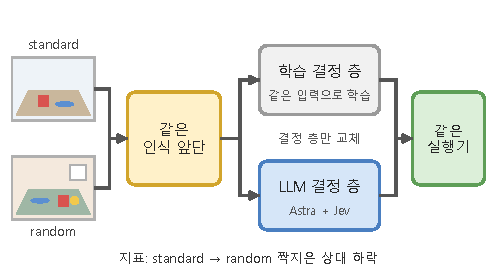
\includegraphics[width=\linewidth]{figures/eval_protocol.pdf}
\caption{\textbf{평가 프로토콜.} 같은 layout의 standard와 random 장면을 짝지어 돌리고 상대 하락(RD)을 잰다. 상위 계획기(Astra, 학습한 8B·35B, 첫 계획 뒤 끔)와 구성(VLA 단독, 상위 단독, 상위 + VLA)을 한 축씩 바꾸고, $\pi_{0.5}$ 미세조정·코드 정책·규칙 기준선을 같은 짝에서 돌린다. 지연 충실 트랙과 동기 공정 트랙을 같은 표에 둔다. 장면 그림은 설명용이다.}
\label{fig:eval}
\end{figure}

주 지표는 같은 layout의 standard와 random을 짝지어 계산한 상대 하락
\begin{equation}
  \mathrm{RD} = 1-\frac{\mathrm{Succ}_{\text{random}}}{\mathrm{Succ}_{\text{standard}}}
\end{equation}
이다(\cref{fig:eval}). 절대 성공률의 우위는 주장하지 않는다. 가설은 셋이며 모두 지연 충실 트랙에서 판정한다. \textbf{H1(시스템 수준)}: $\Delta\mathrm{RD}$(Harvest-B $-$ $\pi_{0.5}$ 미세조정)의 95\% 상한이 0보다 작다. \textbf{H2(학습량)}: 같은 백본의 C, A, A+RL, B의 RD를 비교한다. RD가 학습량과 함께 커지면 ``학습할수록 분포 밖 하락이 커진다''를, 커지지 않으면 그 반대를 보고한다. 어느 쪽이든 결과로 싣는다. \textbf{H3(위층)}: Astra를 첫 계획 뒤 끈 조건의 RD가 켠 조건보다 크다(하한 $>0$). 모듈형 스택에서는 standard에서 random으로 갈 때 인식 술어 정확도가 얼마나 떨어지는지 먼저 재어, 하락이 인식 몫인지를 가른다.

\begin{table*}[t]
\centering
\scriptsize
\setlength{\tabcolsep}{4pt}
\begin{tabular}{@{}lllccccc@{}}
\toprule
범주 & 시스템 & 아래층 학습량 & standard 성공(\%) & random 성공(\%) & RD $\downarrow$ & 정지 시간(s/판) & Astra 호출/판 \\
\midrule
\multirow{5}{*}{기준선}
 & Astra만 (Inspect Robots \texttt{agent})~\cite{inspectrobots2026} & 없음 & \todoexp & \todoexp & \todoexp & \todoexp & \todoexp \\
 & 코드 정책 (CaP-X식)~\cite{fu2026capx} & 없음 & \todoexp & \todoexp & \todoexp & \todoexp & \todoexp \\
 & $\pi_{0.5}$ 미세조정~\cite{pi05_2025} & 전체 & \todoexp & \todoexp & \todoexp & \todoexp & --- \\
 & 룰베이스(같은 상태 위 규칙 + 스크립트 스킬) & 없음 & \todoexp & \todoexp & \todoexp & \todoexp & --- \\
 & 모듈형 스택(명시적 인식 + 결정 A + $S$) & 결정층 & \todoexp & \todoexp & \todoexp & \todoexp & \todoexp \\
\midrule
\multirow{5}{*}{Harvest}
 & C: 영점 결정 토큰 + $S$ & 없음 & \todoexp & \todoexp & \todoexp & \todoexp & \todoexp \\
 & A: 결정층 SFT + $S$ & 결정층 & \todoexp & \todoexp & \todoexp & \todoexp & \todoexp \\
 & A+RL + $S$ & 결정층 & \todoexp & \todoexp & \todoexp & \todoexp & \todoexp \\
 & \textbf{B: 융합 VLA (주 시스템)} & 결정 + 행동 & \todoexp & \todoexp & \todoexp & \todoexp & \todoexp \\
 & B, Astra 첫 계획 뒤 끔 & 결정 + 행동 & \todoexp & \todoexp & \todoexp & \todoexp & 1 \\
\bottomrule
\end{tabular}
\caption{\textbf{주 결과 (계획, 지연 충실 트랙; 동기 공정 트랙은 같은 형식으로 병기).} 기대: 학습 VLA와 결정층을 많이 학습한 조건은 standard 성공률이 높지만 RD가 크고, Harvest-B는 $\pi_{0.5}$ 미세조정보다 RD가 작다(H1). Astra를 끄면 RD가 커진다(H3). 학습량 축(C, A, A+RL, B)의 RD 순서는 학습이 분포 밖 하락을 키우는지(H2)를 보여 준다. 정지 시간은 첫 계획과 안전 대기 밖에서 0이어야 하며, 아니면 구현 결함으로 재실행한다.}
\label{tab:main}
\end{table*}

\subsection{Astra 호출 주기 (E-M8c)}
처음에는 하트비트 주기 $N$을 정하는 실험으로 등록했다. \cref{sec:astra}의 역할 재정의 뒤에는 현재 구현인 하트비트(K2-$N$)가 기준선이 되고, 저빈도 감사와 ``작은 층이 모를 때만'' 호출하는 정책(K5)을 이 표에 더해 새 사전 등록으로 비교한다. K5가 K2-$N$ 최선보다 성공률이 \tentative{$-2$\%p} 안에서 비열등(하한 \tentative{$>-4$\%p})이고 실패가 아닌 Astra 호출이 \tentative{50\%} 이상 줄면 런타임 기본을 K5로 바꾼다(판정 초안). 원래 조건은 K0(첫 계획, 실패, 사건만), K1(K0 + 단계 경계), K2-$N$(K1 + 하트비트, $N\in\{0,5,10,20\}$\,s), K3(Gemini 하트비트 원문 충실판~\cite{geminier_docs2026}), K4(호출 수를 맞춘 사건 전용 대조)이다. critic이 실패를 내지 않는 ``감시기 밖 실패'' 섭동을 반드시 포함한다. 사전 판정: K2-$N$$-$K1이 \tentative{+3\%p} 이상이고 하한 $>0$이면 하트비트를 채택하고, 최고 조건 대비 \tentative{$-2$\%p} 안에서 가장 큰 $N$을 기본값으로 쓴다. API 모델은 같은 입력에도 답이 흔들리므로, 반복 실행 수를 검정력 계산으로 미리 정한다. 과제 중 연속 감독을 직렬 흐름으로 바꾼 뒤(\cref{sec:stream})에는 이 표가 흐름 밖 트리거 호출의 설계를 정하고, 흐름 자체의 가치는 E-Couple(\cref{sec:plan_couple})이 잰다.

\begin{table}[t]
\centering
\scriptsize
\setlength{\tabcolsep}{3pt}
\begin{tabular}{@{}lcccc@{}}
\toprule
조건 & 성공(\%) & \makecell{감시기 밖\\실패 회복(\%)} & 호출/판 & \makecell{비용\\(\$/판)} \\
\midrule
K0 첫 계획 + 실패 + 사건 & \todoexp & \todoexp & \todoexp & \todoexp \\
K1 K0 + 단계 경계 & \todoexp & \todoexp & \todoexp & \todoexp \\
K2-0 K1 + 하트비트 $N{=}0$\,s & \todoexp & \todoexp & \todoexp & \todoexp \\
K2-5 (현재 구현) & \todoexp & \todoexp & \todoexp & \todoexp \\
K2-10 & \todoexp & \todoexp & \todoexp & \todoexp \\
K2-20 & \todoexp & \todoexp & \todoexp & \todoexp \\
K3 Gemini 하트비트 충실판 & \todoexp & \todoexp & \todoexp & \todoexp \\
K4 호출 수 맞춘 사건 전용 & \todoexp & \todoexp & \todoexp & \todoexp \\
\textbf{K5 감사 + 모를 때만} & \todoexp & \todoexp & \todoexp & \todoexp \\
\bottomrule
\end{tabular}
\caption{\textbf{Astra 호출 주기 (계획).} 기대: 감시기 밖 실패의 회복률은 하트비트를 더한 K2가 K1보다 높지만, 저빈도 감사와 ``모를 때만'' 호출하는 K5가 호출을 크게 줄이면서 같은 회복률을 낸다. 성립하면 역할 재정의(\cref{sec:astra})를 지지한다. K5가 비열등하지 않으면 하트비트를 기준선이 아니라 기본으로 되돌리고 그 결과를 그대로 보고한다. K5 행은 새 사전 등록으로 더한다.}
\label{tab:hb}
\end{table}

\subsection{이미지 입력 절제와 E-CAM3}
\label{sec:plan_img}
결정층에 어떤 카메라를 넣을지 정한다. 공개 실물 데이터에서 먼저 도는 \textbf{E-CAM3}는 S-E2E 고친 데이터(\texttt{se2e\_c1})에서 \{머리 + 활성 손목, 머리 + 두 손목\}을 움직임 줄을 켠 채 같은 스케줄로 비교하고, E-TC와 같은 틀(전체 정확도 $\ge+0.02$, 전환 층 $\ge-0.01$, decide p95 증가 $\le10\%$)로 채택한다. 공개 데이터에는 두 손목 영상이 모두 있었다(기준이 쓰는 \tentative{39,283}행 전부, 빠짐 0). \textbf{E-CAM3 결과(끝, 불채택)}: 검증 전체 1,799 스냅샷에서 두 시드 합동 효과 \tentative{+0.0014}(95\% 구간 \tentative{[$-$0.0041, +0.0069]}), 전환 층 \tentative{+0.0016}, FULL 결정 p95 \tentative{+11.7\%}(84.6 $\rightarrow$ 94.6\,ms; 늘어난 몫은 주로 세 번째 이미지의 읽기·전처리)로 채택 조건 셋을 못 넘었고, 시드별 효과의 부호도 갈렸다(\tentative{+0.0044}, \tentative{$-$0.0017}). 그래서 결정 입력은 머리 + 활성 손목을 유지하고, 두 손목은 Astra 요청에만 쓴다(정본 §57 보충). 아래 시뮬 절제는 카메라가 정확한 데이터에서 같은 질문을 접촉 구간별로 다시 본다. 조건은 머리만, 머리 + 활성 손목 상시, 머리 + 활성 손목(근접·접촉 구간만), 머리 + 두 손목이다. 모듈형 입력에서는 좌표를 참값으로 주면 이미지 효과가 가려지므로(예비 시험에서 참값 좌표 위의 이미지 이득은 \tentative{+0.0001}이었다), 인식 추정 잡음이 든 좌표 조건을 주 판정으로 둔다. 융합 입력(좌표 없음)에서도 같은 네 조건을 잰다. 지표는 결정 정확도(특히 \texttt{mag}와 접촉 구간)와 p95 지연이다.

\begin{table}[t]
\centering
\scriptsize
\setlength{\tabcolsep}{1.8pt}
\begin{tabular}{@{}lccccc@{}}
\toprule
& \multicolumn{3}{c}{모듈형(추정 좌표 잡음)} & 융합 & \\
\cmidrule(lr){2-4}\cmidrule(lr){5-5}
이미지 & 정확도 & \texttt{mag} & 접촉 구간 & 정확도 & p95 (s) \\
\midrule
머리만 & \todoexp & \todoexp & \todoexp & \todoexp & \todoexp \\
머리 + 활성 손목(상시) & \todoexp & \todoexp & \todoexp & \todoexp & \todoexp \\
머리 + 활성 손목(근접·접촉) & \todoexp & \todoexp & \todoexp & \todoexp & \todoexp \\
머리 + 두 손목 & \todoexp & \todoexp & \todoexp & \todoexp & \todoexp \\
\bottomrule
\end{tabular}
\caption{\textbf{결정층 이미지 절제 (계획).} 공개 실물 데이터의 E-CAM3(머리 + 두 손목, 불채택)는 본문에 적었다. 기대: 활성 손목을 넣으면 \texttt{mag}와 접촉 구간 정확도가 오르고, 두 손목을 모두 넣는 것은 지연만 늘린다. 성립하면 기본 입력(머리 + 활성 손목)을 지지한다. 기간 안의 손목 카메라 단독 절제 근거는 찾지 못했으므로 이 실험이 우리 근거가 된다.}
\label{tab:img}
\end{table}

\subsection{보정 (E1)}
\label{sec:plan_e1}
보정 자료는 CAL 편을 편 id 해시 순서로 둘로 나눠 한쪽은 질문별 온도, 다른 쪽은 conformal 문턱에 쓴다. 질문군마다 보정 뒤 ECE $\le$ \tentative{0.05}(15개 동일 질량 구간, 애매한 항목 제외, 부트스트랩 상한 $\le$ \tentative{0.08}), 정오답 판별 AUROC $\ge$ \tentative{0.75}, 보정 확률 $\ge\theta$ 구간의 실제 정확도 $\ge\theta-0.03$을 모두 만족할 때만 확률 게이트를 켠다. conformal 게이트는 $\alpha\in\{0.05,0.1,0.2\}$에서 커버리지 하한이 $1-\alpha-0.03$ 이상이고 원소 하나 비율이 \tentative{50\%} 이상인 질문군에서만 켠다. random에서 커버리지가 떨어지는 것 자체가 결과이며(교환 가능성 가정이 깨짐), RD와 함께 보고한다. 모든 질문군이 실패해도 설계는 최빈 선택만으로 선다.

\subsection{소규모 end-to-end 학습 (S-E2E, 파이프라인 판정)}
\label{sec:plan_se2e}
실물 공개 데이터로 융합 모델(단계 B) 학습이 끝까지 돌고, 손실이 줄고, 저장·재적재·재개가 정확한지를 본다. 과제 성공은 보지 않으며(롤아웃 없음) 수치는 결과로 쓰지 않는다. 설정은 ROBOTIS AI Worker 두 과제의 학습 표본 37,484개, 묶음 8로 1 에폭(4,686스텝), 두 시드(0, 1)이다. 이 데이터에는 보조·확인 라벨이 없어 실제 학습 신호는 결정 NLL과 flow matching뿐이다. 판정은 출처별로 층화한 검증 부분집합 300개에서, 시드마다 (a) 완주와 모든 손실의 유한성, (b) 감소(마지막 세 평가점 평균이 처음 대비 결정 NLL \tentative{$\le 0.70\times$}, flow matching \tentative{$\le 0.80\times$}, 샘플 청크 오차 \tentative{$\le 0.80\times$}; 마지막 한 점도 결정 NLL \tentative{$\le 0.80\times$}, flow matching \tentative{$\le 0.90\times$}), (c) 끝과 중간(2,000스텝) 체크포인트의 재적재 일치(행동 차 0.0, 평가 값 동일), (e) 2,000스텝에서 재개한 50스텝의 재현(비트 동일, 또는 데이터 순서·스케줄이 같고 총손실 상대차 중앙값 \tentative{$\le1\%$}·최댓값 \tentative{$\le5\%$})를 보고, 두 시드가 모두 통과해야 통과다. 비트 동일 대신 허용치를 둔 이유는 같은 체크포인트에서 두 번 재개한 판끼리도 GPU 역전파 비결정성으로 같은 크기만큼 어긋났기 때문이다. 판정 스크립트는 학습이 끝나기 전에 저장소에 고정했고, 문턱은 사전 등록 그대로 두고 두 가지만 정했다. ``$\le$'' 비교에 상대 허용 $10^{-12}$를 둔다(끝 세 점 0.65, 0.65, 0.80의 평균이 부동소수로 0.7000000000000001이 되어 0.70 문턱에서 떨어지던 문제). (a)의 종료 코드는 학습 구동기의 출력에서 직접 읽는다. 판정은 이 판본으로만 한다. 학습은 사전 등록 직후 두 시드로 시작했다. 이 학습은 (b) 되먹임 줄을 넣기 전의 입력 형식으로 고정한 코드 사본으로 돌고 판정도 그 사본으로 한다. S-E2E의 결정 항목은 원래 자체 문맥을 쓰는 파이프라인 시험이라 새 형식과 무관하며, 이 체크포인트는 폐루프에 쓰지 않는다.

\paragraph{파이프라인 확인 통과.} 두 시드 모두 (a), (b), (c)를 통과했고 (e)는 허용 기준으로 통과해(비트 동일은 아님; 재개 첫 스텝 손실은 같고 총손실 상대차 중앙값 \tentative{0.46\%, 0.39\%}), 사전 등록 판정이 \emph{통과}였다. 검증 결정 NLL은 \tentative{4.62에서 0.68과 0.69}로, flow matching 손실은 \tentative{2.2--2.4에서 0.06과 0.05}로 줄었고, 결정 정확도는 \tentative{약 0.72}였다. 학습과 검증의 결정 NLL이 거의 같아 과적합은 보이지 않았다. GPU 사용률은 평균 \tentative{약 46\%}에 그쳤는데, 같은 시간에 파드 CPU 할당량이 거의 찼으므로 이미지 적재·전처리가 CPU에 묶인 것으로 보인다(원인 미측정). 이 수치는 모두 파이프라인 확인이며 결과로 쓰지 않는다.

\paragraph{정확도 진단(사전 등록).} 정확도 \tentative{0.72}의 원인을 가르려고 결과를 보기 전에 세 진단을 등록했다. (D1) 끝 체크포인트에서 상수 학습률로 \tentative{1,200스텝}을 더 돌려도 검증 결정 NLL이 문턱 아래로 내려가지 않아 ``이 학습률에서는 계산 한계가 아님''으로 판정했다. 앞선 개선은 대부분 학습률 감쇠 구간에서 나왔다. (D2) 학습 표본 1,000개로 과적합 시험을 하면 학습 부분집합 정확도가 \tentative{0.885}(검증 \tentative{0.56})로 사전 등록 구간 안에 들어 ``불확정''이었다. (D3) 오답 가운데 라벨 경계 근처 표본은 \tentative{34\%}로 문턱 50\%에 못 미쳐 ``라벨 모호성 한계가 아님''이었다. 0.1\,s 떨어진 이웃 프레임끼리 라벨이 달라지는 비율로 잡은 단일 프레임 정확도의 대략 상한은 \tentative{약 0.93}이다. 오답은 대부분 ``움직이는가''와 크기 한 칸 차이였고, 방향 부호가 반대인 경우는 드물었다(\tentative{8/155}). 이 시점의 종합 판정은 \emph{판정 불가}였다. 이어서 등록한 규모 곡선(아래)의 $N{=}1{,}000$ 판에서 학습 부분집합 정확도가 \tentative{1.000}, 검증이 \tentative{0.552}여서 D2는 원래 규칙대로 ``라벨은 학습 가능, 일반화 간극''으로 해소됐다(스케줄이 원래 D2와 다름). 그러면 종합 칸은 ``데이터 규모 한계 $\rightarrow$ 데이터 늘리기''가 되지만, 같은 스텝 규모 곡선이 이 처방의 범위를 약 9k 표본까지로 제한한다. 남은 레버는 시간 맥락(\cref{sec:plan_temporal})과 더 긴 감쇠 스케줄이다. 이 진단 수치도 파이프라인 시험의 것이라 결과로 쓰지 않는다.

\paragraph{같은 스텝 데이터 규모 곡선(사전 등록 추가).} 진단 결과를 본 뒤, 실행 전에 ``데이터를 늘리면 결정 정확도가 오르는가''를 같은 계산량에서 재는 곡선을 추가로 등록했다. 학습 표본 $N$을 1,000(D2와 같은 부분집합), 9,371(25\%), 18,742(50\%), 37,484(100\%)로 두고, 네 판 모두 기반 모델에서 새로 같은 2,000스텝(묶음 8, 학습률 $10^{-4}$, 워밍업 3\% 뒤 코사인, 시드 0)을 돌린다. 25\%와 50\%는 출처별로 같은 비율이며 25\%가 50\%에 포함된다. 검증은 S-E2E와 같은 층화 300개다. step 2,000의 검증 결정 정확도에 $\text{acc}=a+b\log_{10}N$을 최소제곱으로 맞추고, $b\ge$ \tentative{0.05}(10배당)이면서 $\text{acc}(100\%)-\text{acc}(25\%)\ge$ \tentative{0.03}이면 ``데이터 규모 레버 확인'', $\text{acc}(100\%)-\text{acc}(50\%)<$ \tentative{0.01}이면 ``포화''를 함께 표시하고, 둘 다 아니면 ``레버 약함(같은 스텝 기준)''으로 읽는다. $+0.05$에 필요한 $N$의 외삽과 NLL 곡선은 판정 밖으로 보고한다. 같은 스텝이라 $N{=}1{,}000$은 16 에폭을, 100\%는 0.43 에폭을 보므로 이 곡선은 같은 계산에서의 데이터 다양성 효과다. $N{=}1{,}000$ 판의 학습 부분집합 정확도로 D2를 원래 규칙대로 다시 판정한다(스케줄이 D2와 다르다는 점을 함께 적는다).

\paragraph{규모 곡선 결과(사전 등록 판정).} step 2,000의 검증 정확도는 $N$ = 1,000, 9,371, 18,742, 37,484에서 \tentative{0.552, 0.682, 0.686, 0.683}이었다(\cref{tab:scale}). 적합 기울기는 \tentative{$b=0.090$}으로 문턱을 넘지만, $\text{acc}(100\%)-\text{acc}(25\%)=$ \tentative{$+0.001$}이라 ``확인'' 조건을 채우지 못했고, $\text{acc}(100\%)-\text{acc}(50\%)=$ \tentative{$-0.002$}라 포화 표시가 붙었다. 판정은 ``데이터 규모 레버 약함(같은 스텝 기준), 50\%$\rightarrow$100\% 포화''다. 기울기는 16 에폭 과적합 판인 $N{=}1{,}000$ 한 점이 만든 것이고 위 세 점은 평평하므로, $+0.05$에 필요한 $N$의 외삽(\tentative{약 13만})은 믿을 근거가 약하다. 판정 밖 읽기로, $N{=}9{,}371$ 판은 학습 부분집합과 검증 정확도가 거의 같아(\tentative{0.706} 대 \tentative{0.682}) 과소적합 영역이다. 이 계산량에서는 약 9k 표본을 넘는 다양성이 정확도를 올리지 않았고, 데이터보다 스텝이 막고 있다. 이 곡선은 입력(시간 맥락 부재)이 정하는 한계라는 가설과도 충돌하지 않는다.

\begin{table}[t]
\centering
\scriptsize
\setlength{\tabcolsep}{3pt}
\begin{tabular}{@{}rcccc@{}}
\toprule
학습 표본 $N$ & 에폭 & 검증 정확도 & 검증 결정 NLL & 학습 부분집합 정확도 \\
\midrule
1,000 & 16 & \tentative{0.552} & \tentative{5.342} & \tentative{1.000} \\
9,371 (25\%) & 1.7 & \tentative{0.682} & \tentative{0.796} & \tentative{0.706} \\
18,742 (50\%) & 0.85 & \tentative{0.686} & \tentative{0.768} & --- \\
37,484 (100\%) & 0.43 & \tentative{0.683} & \tentative{0.773} & --- \\
\midrule
\multicolumn{5}{@{}l}{기울기 $b$ (10배당) \tentative{0.090} \quad 판정: 레버 약함(같은 스텝), 50\%$\rightarrow$100\% 포화} \\
\bottomrule
\end{tabular}
\caption{\textbf{같은 2,000스텝 데이터 규모 곡선 (사전 등록 판정, 파이프라인 시험).} 기대는 정확도가 $\log_{10}N$에 따라 오르고 100\%에서도 포화하지 않는 것이었다. 결과는 1,000에서 9,371로는 크게 오르고 그 위에서는 평평해, 같은 계산에서 데이터 다양성은 약 9k 표본까지만 듣는다. 남은 원인은 입력 쪽(\cref{sec:plan_temporal})과 계산(더 긴 감쇠)으로 돌린다. $N{=}1{,}000$의 NLL은 16 에폭 과적합 값이다. 학습 부분집합 정확도는 $N{=}9{,}371$에서 그 안의 층화 1,000개로 쟀다. 공개 데이터의 휴리스틱 라벨이라 수치는 논문 결과로 쓰지 않는다.}
\label{tab:scale}
\end{table}

\subsection{시간 맥락 시험 (E-TC, 사전 등록 판정)}
\label{sec:plan_temporal}
\cref{sec:temporal}의 과거 프레임 입력과 움직임 줄이 결정 정확도를 올리는지를 본다. 설계, 지표, 층 정의, 문턱, 판정 스크립트는 어느 칸도 학습하기 전에 사전 등록했다. 같은 공개 데이터(학습 37,484, 검증은 S-E2E와 같은 층화 300), 같은 스케줄(2,000스텝, 묶음 8, 학습률 $10^{-4}$, 워밍업 3\% 뒤 코사인, 부분집합 없이 약 0.43 에폭)에서 두 요인을 교차한 2$\times$2로 기반 모델에서 새로 학습한다. 요인 V는 이미지 입력(한 시점 대 카메라마다 $[t-0.3\,\text{s},\,t]$ 2프레임 비디오), 요인 M은 움직임 줄(없음 대 있음, \cref{sec:temporal})이다. 움직임 줄은 팔 속도 세 구간과 그리퍼 열림·닫힘만 담고 방향은 담지 않으며, 학습 때 표본마다 확률 \tentative{0.3}으로 값을 \texttt{unknown}으로 바꾼다. 두 요인을 한 격자에서 재는 이유는 둘이 같은 정보(속도)를 다른 경로로 주기 때문이다. 시드는 \tentative{하나(0)}이고, 두 번째 시드, $\Delta=0.1$\,s 칸, 과거 프레임 드롭아웃은 이번 등록 범위 밖이다. 옵션 판은 기본 경로와 프롬프트 판본 해시가 걸린 파일을 바꾸지 않고 새 판본 표지를 해시에 더한다. (한 시점, 줄 없음) 칸은 새로 돌리지 않고 데이터 규모 곡선의 100\% 판을 재사용한다. 설정이 같고, 옵션을 끈 경로가 같은 표본과 같은 스텝 함수를 쓰기 때문이다. 재사용 조건은 그 판의 인자가 위 값과 같고, 정상 종료, step 2,000 평가와 끝 체크포인트가 있으며, 이 시험의 코드 사본으로 다시 돌린 예측 요약이 그 판의 step 2,000 평가 기록과 같은 것이다. 다르면 이 칸을 이 사본으로 새로 돌린다. 재사용 조건은 모든 필드에서 통과했고, 나머지 세 칸은 데이터 규모 판이 끝난 뒤 학습했다.

지표는 각 칸의 step 2,000 체크포인트로 검증 300개 $\times$ 세 질문 = 900항목에서 잰 결정 정확도와 결정 NLL(질문 보기 집합 안에서 재정규화한 $-\log p$(정답))이며, 전체와 \textbf{전환 층}에서 잰다. 스냅샷 $k$는 어느 질문이든 프레임 단위 라벨이 $k$와 $k+j$($j=1,2,3$, 곧 0.1--0.3\,s, 다음 결정까지 0.33\,s의 10\,Hz 최근접)에서 하나라도 다르면 전환 층이다. 스냅샷 경계 표시(``다음 결정 스냅샷과 술어가 바뀜'')를 공개 데이터 라벨로 옮긴 정의이며, 라벨만으로 계산해 검증 행의 \tentative{65.1\%}가 전환 층이다. 층이 이렇게 크다는 점은 결과 전에 적어 두었다. 나머지는 정상 층이다. 질문별 정확도, 질문별 전환 층, 스냅샷 군집 부트스트랩 95\% 구간(10,000회)은 판정 밖으로 보고한다. 전환 층을 따로 보는 이유는 GAP~\cite{gap2026}의 보고 때문이다. 시각과 고유감각을 단순히 이어 붙인 정책은 움직임 전환 구간에서 시각을 덜 쓰게 되어 시각만 쓴 정책보다 나빠질 수 있었다. 속도 입력은 ``지금 움직이면 다음에도 움직인다''는 지름길을 주므로, 정상 층 점수는 오르면서 우리가 고치려는 전환 순간은 나빠질 수 있다. decide 지연은 모든 학습이 끝난 뒤 한 H200에서, 머리와 손목 한 대를 쓰는 검증 표본 50개로 네 형식을 번갈아(워밍업 30회 뒤 형식마다 200회) 잰다. 판정에는 이미지 읽기, 전처리(비디오는 두 프레임), 토큰화, GPU 순전파를 모두 포함한 p95를 쓴다. 런타임은 과거 프레임 전처리를 앞 호출에서 재사용할 수 있으므로 보수적인 값이다.

채택 규칙(사전 등록)은 요인마다 따로 적용한다. 칸 정확도를 $a_{VM}$($V\in\{s,v\}$는 한 시점과 비디오, $M\in\{0,1\}$은 줄 없음과 있음)이라 하면 V의 주효과는 $\tfrac12[(a_{v0}-a_{s0})+(a_{v1}-a_{s1})]$, M의 주효과는 $\tfrac12[(a_{s1}-a_{s0})+(a_{v1}-a_{v0})]$, 상호작용은 $(a_{v1}-a_{v0})-(a_{s1}-a_{s0})$이다. 요인은 (1) 전체 정확도 주효과가 \tentative{$+0.02$} 이상, (2) 전환 층 정확도 주효과가 \tentative{$-0.01$} 이상, (3) decide p95 증가가 \tentative{10\%} 이하(V는 (비디오, 없음) 대 (한 시점, 없음), M은 (한 시점, 있음) 대 (한 시점, 없음))일 때만 채택한다. 상호작용과 NLL 주효과는 판정 밖으로 보고한다. 검증 300개에서 정확도 표준오차는 약 \tentative{0.02--0.03}으로 문턱보다 크다는 점도 미리 적었으며, 판정은 규칙대로 내고 구간을 함께 보고한다. 판정 스크립트는 문턱을 상수로 담아 결과 전에 저장소에 고정했다. (비디오, 없음) 칸이 먼저 끝나면 기준 대비 단순 효과를 판정 밖으로 먼저 보고하고, 채택 판정은 네 칸이 끝난 뒤에만 한다. V가 채택되지 않으면 기본 입력은 한 시점으로 두고, 그 결과를 이 표에 그대로 보고한다. 이 시험도 공개 데이터의 휴리스틱 라벨을 쓰는 소규모 학습이라, 채택은 본 단계 B 입력 형식을 정하는 근거일 뿐 논문 결과는 본 데이터로 다시 잰다.

\paragraph{판정.} 사전 등록 규칙과 결과 전에 고정한 판정 스크립트를 그대로 적용했다(\cref{tab:temporal}). \textbf{움직임 줄(M)은 채택}이다. 전체 정확도 주효과 \tentative{$+0.025$}(95\% 구간 \tentative{$[+0.003, +0.047]$}), 전환 층 \tentative{$+0.027$}, decide p95 \tentative{$-3.8\%$}로 세 조건을 모두 통과했다. \textbf{2프레임 비디오(V)는 채택하지 않는다}. 전체 주효과가 \tentative{$+0.013$}으로 문턱 $+0.02$에 못 미쳤고, 전처리를 포함한 p95가 \tentative{$+20.4\%$} 늘었다. 판정 밖으로 읽으면, V는 모든 층에서 NLL을 낮추었고 지연 증가는 모두 과거 프레임을 매번 읽는 CPU 전처리 몫이었다(GPU 순전파 p95는 \tentative{$-0.9\%$}). 앞 호출의 전처리 프레임을 재사용하는 판과 $\Delta=0.1$\,s 칸은 새 사전 등록으로만 다시 잰다. 상호작용은 모든 층에서 구간이 0을 포함했다. M은 GAP식 전환 층 악화 없이 전체와 전환 층을 함께 올렸고, 이득은 주로 크기 질문(\texttt{mag})에 모였다. 이는 진단 D3의 ``움직이는가, 크기 한 칸'' 오답 유형과 맞는다. 두 요인을 합친 칸은 기준보다 전체 \tentative{$+0.038$}, 전환 층 \tentative{$+0.045$}였다(서술만). 시드 하나, 검증 300개라 M 구간의 하한이 0에 가깝고, 칸 차이의 일부는 학습 잡음일 수 있다. 채택 뒤 공개 데이터 행의 고유감각 속도가 중앙 차분(0.1\,s 미래 포함)이라는 누수를 찾았다(\cref{sec:temporal}). 움직임 줄은 이 값을 쓰지 않았으므로 판정은 유지하되, 누수를 고친 데이터로 확인 실험을 새로 등록했다(아래). 지연은 학습 코드의 HF 순전파로 잰 값이라 융합 서버의 decide(약 \tentative{0.33\,s})와 절대값이 다르며 비율만 판정에 썼다.

\begin{table}[t]
\centering
\scriptsize
\setlength{\tabcolsep}{2.5pt}
\begin{tabular}{@{}lccccc@{}}
\toprule
이미지 입력 & 움직임 줄 & 전체 & 전환 층 & 정상 층 & p95 (s) \\
\midrule
한 시점(기준)$^\dagger$ & 없음 & \tentative{0.683} & \tentative{0.612} & \tentative{0.828} & \tentative{0.098} \\
한 시점 & 있음 & \tentative{0.708} & \tentative{0.632} & \tentative{0.862} & \tentative{0.095} \\
2프레임 비디오 & 없음 & \tentative{0.696} & \tentative{0.624} & \tentative{0.842} & \tentative{0.118} \\
2프레임 비디오 & 있음 & \tentative{0.721} & \tentative{0.657} & \tentative{0.852} & \tentative{0.123} \\
\midrule
\multicolumn{2}{@{}l}{주효과 V (비디오): 불채택} & \tentative{+0.013} & \tentative{+0.018} & \tentative{+0.002} & \tentative{+20.4\%} \\
\multicolumn{2}{@{}l}{주효과 M (움직임 줄): 채택} & \tentative{+0.025} & \tentative{+0.027} & \tentative{+0.022} & \tentative{$-$3.8\%} \\
\multicolumn{2}{@{}l}{상호작용 V$\times$M (판정 밖)} & \tentative{+0.001} & \tentative{+0.013} & \tentative{$-$0.024} & --- \\
\bottomrule
\end{tabular}
\caption{\textbf{시간 맥락 2$\times$2 (사전 등록 판정, 파이프라인 시험).} 값은 검증 300개 $\times$ 세 질문의 결정 정확도, 시드 0, p95는 전처리를 포함한 decide 지연(학습 코드의 HF 순전파, 비율만 판정에 씀). $^\dagger$데이터 규모 곡선의 100\% 판 재사용(\cref{tab:scale}). 주효과의 p95 열은 V는 (비디오, 없음), M은 (한 시점, 있음)을 기준 칸과 비교한 증가율이다. 기대는 2프레임 비디오가 p95를 거의 바꾸지 않으면서 정확도를 올리고, 움직임 줄은 전환 층에서 손해일 수 있다는 것이었다. 결과는 반대였다. 움직임 줄이 전환 층을 포함해 규칙을 통과했고, 비디오는 정확도 이득이 문턱 아래였으며 CPU 전처리로 p95가 늘었다. 한 시점 입력의 속도 부재가 결정 오답의 한 원인이라는 가설은 텍스트 경로로 지지되며, 누수를 고친 데이터의 두 시드 확인에서도 유지되었다(\cref{tab:motionconfirm}). 판정은 입력 형식 선택에만 쓴다.}
\label{tab:temporal}
\end{table}

\paragraph{움직임 줄 확인 실험(사전 등록 판정).} E-TC의 채택이 시드 하나와 검증 300개에 기대므로, 결과를 보기 전에 확인 규칙을 등록했다. 누수를 고친 데이터(\texttt{se2e\_c1})에서 움직임 줄 없음·있음을 시드 1과 2로 각각 같은 2,000스텝 학습하고, 검증 전체 1,799개 $\times$ 세 질문으로 잰다. 채택 확인은 두 시드의 짝 효과 평균(합동 효과)이 $\ge+0.015$이고 95\% 하한이 0보다 크며(엄격한 부등호), 전환 층 합동 효과가 $\ge-0.01$일 때다. 결과는 합동 \tentative{+0.032} \tentative{[+0.022, +0.043]}, 전환 층 \tentative{+0.030} \tentative{[+0.016, +0.043]}, 정상 층 \tentative{+0.037}로 확인되었다(\cref{tab:motionconfirm}). 두 시드의 효과 차는 \tentative{0.004}로 작았고, NLL은 모든 층에서 줄었다. 판정 밖으로 검증 300개 부분집합만 보면 합동 \tentative{+0.026} \tentative{[$-$0.001, +0.052]}로 하한이 0에 걸쳐, 처음 판정의 구간이 좁지 않았던 것이 표본 크기 때문이었음을 보여 준다.

\begin{table}[t]
\centering
\scriptsize
\setlength{\tabcolsep}{4pt}
\begin{tabular}{@{}lccc@{}}
\toprule
& 시드 1 & 시드 2 & 합동 (95\% 구간) \\
\midrule
움직임 줄 없음 & \tentative{0.672} & \tentative{0.677} & --- \\
움직임 줄 있음 & \tentative{0.707} & \tentative{0.708} & --- \\
효과(전체) & \tentative{+0.034} & \tentative{+0.030} & \tentative{+0.032 [+0.022, +0.043]} \\
효과(전환 층) & --- & --- & \tentative{+0.030 [+0.016, +0.043]} \\
\bottomrule
\end{tabular}
\caption{\textbf{움직임 줄 확인 (사전 등록 판정, 파이프라인 시험).} 누수를 고친 데이터, 두 시드, 검증 전체 1,799개 $\times$ 세 질문의 결정 정확도. 등록 규칙(합동 $\ge+0.015$, 하한 $>0$, 전환 층 $\ge-0.01$)을 모두 통과해 채택이 확인되었다. 공개 데이터의 휴리스틱 라벨이라 수치는 입력 형식 선택에만 쓴다.}
\label{tab:motionconfirm}
\end{table}

\subsection{MolmoAct식 궤적 실험 (E-MA1, E-MA1b, E-MA2, E-MA3)}
\label{sec:plan_molmo}
\paragraph{E-MA1과 관문 G0 (실패).} 처음 등록한 E-MA1은 미래 궤적 보조 손실(A: 머리 영상 위 5점) $\times$ 손끝 이력 덧그림(O: 머리 영상, 과거 2\,s)의 2$\times$2였다. 둘 다 머리 카메라로의 FK 투영이 맞아야 하므로, 학습 전 관문 G0에서 검증 분할 머리 프레임 120장의 투영을 VLM 포인팅(Molmo2-ER) 기준점과 비교했다. 통과 조건은 오차 중앙값 $\le12$\,px이고 90분위 $\le30$\,px였다. 유효 기준점 \tentative{119장}에서 명목 카메라 모델은 중앙값 \tentative{100.9\,px}, 90분위 \tentative{264.5\,px}였고, 원천별 PnP 보정 뒤 검사 반쪽(\tentative{59장})에서도 \tentative{86.9\,px}와 \tentative{212.1\,px}로 실패했다. 한 원천은 머리 관절이 기록되지 않아 머리 각을 고정 가정했는데, 그 원천 투영의 절반가량이 영상 아래로 벗어나 이 가정이 주원인으로 보인다. 등록 규칙은 시뮬 데이터로 옮기는 것이지만 R2 학습 데이터가 아직 생성 중이라 규칙대로 멈췄다. 학습한 칸은 없다.

\paragraph{E-MA1b: 로봇 기준 3D 궤적 보조 손실 (끝, 불채택).} 카메라가 필요 없는 형태로 다시 설계했다. 보조 목표는 로봇 기준 좌표계에서 현재 손끝에 대한 미래 손끝 5점의 변위(\texttt{a3d@v1})이며, 실행 경로는 바이트 단위로 바뀌지 않아야 한다. 기준 칸은 움직임 줄 확인 실험의 두 체크포인트(움직임 줄 있음, 시드 1·2)를 그대로 쓰고, 보조 손실을 켠 판만 같은 스케줄로 두 시드 학습한다. 채택은 검증 전체에서 두 시드 합동 효과 $\ge+0.02$, 95\% 하한 $>0$, 전환 층 $\ge-0.01$일 때다. 이 목표는 결정 라벨과 같은 정보를 연속값으로 담으므로 원천별 정확도를 함께 보고하고, 채택되어도 일반화의 근거로 쓰지 않는다. 결과: 합동 효과 \tentative{+0.0031}(95\% 구간 \tentative{[$-$0.0022, +0.0085]}), 전환 층 \tentative{0.0000}으로 불채택이다. 보조 머리는 배웠지만 조금만 배웠다(평균 오차 \tentative{9.9/9.5\,cm}, ``변위 0'' 기준 \tentative{12.4\,cm}). 같은 정보의 연속값 감독이 이 규모(2,000스텝, $\lambda$ 0.1)에서 결정 정확도를 올리지 않는다는 뜻이며, 이미지 좌표 궤적(\texttt{trace5})과 이력 덧그림은 R2 시뮬에서 E-MA1을 다시 등록해 본다.

\paragraph{E-MA2: VLA가 Astra 명령을 따르는가 (끝, NONE).} 명령 없음(C0), 한 줄 문장 \texttt{edit: dx dy dz cm}(C1), 머리 영상 위 두 점 화살표(C2)를 같은 스케줄로 학습한다. 명령은 되짚기(다음 1\,s의 실제 말단 변위를 명령 범위로 자른 것)이며 학습 표본의 절반에만 준다. 평가는 명령 없는 입력의 결정 정확도(비열등)와, 참 명령을 수평면에서 90$^\circ$·180$^\circ$ 돌린 반사실 명령의 준수율(예측 방향이 명령과 같은 칸이고 0.5\,s 청크 변위와 명령의 코사인 $>0.5$)이다. C2 채택은 준수율 C2$-$C1 $\ge+0.10$, 명령 없는 정확도 C2$-$C0 $\ge-0.01$, p95 증가 $\le10\%$일 때다. C1과 C2의 준수율이 모두 0.6 미만이면 VLA는 명령을 보지 않고 코드 편향만 쓴다. 결과(R2 평가 스냅샷 1,200개): 준수율은 C0 \tentative{0.0008}, C1 \tentative{0.177}, C2 \tentative{0.0008}로 둘 다 0.6 미만이라 등록 규칙에 따라 NONE이다(C2$-$C1 \tentative{$-$0.176} [\tentative{$-$0.198, $-$0.155}]). 명령 없는 정확도는 C0 \tentative{0.939}에 대해 C1 \tentative{$-$0.016}, C2 \tentative{$-$0.010}, FULL p95는 \tentative{96.0/95.8/91.0\,ms}였다. C1의 결정층은 돌린 명령에서도 명령 칸을 \tentative{0.970}으로 골랐지만, 그 결정을 조건으로 받은 청크는 \tentative{0.275}(90$^\circ$), \tentative{0.093}(180$^\circ$)만 따랐다. 그래서 ``결정 토큰이 청크를 조종한다''고 가정하지 않고, 준수는 청크 수준에서 잰다(\cref{sec:plan_adh}).

\paragraph{E-MA3: 층별 KV 조건 (끝, 불채택).} expert 블록마다 백본 층 3·8·12·17·21·26·30·35의 K·V에 교차 주의하는 판을 같은 틀로 비교했다. 사전 등록 규칙(1차 지표를 행동 청크 오차로 바꿔 등록): 합동 상대 감소 $\ge5\%$(시드 간 변동 3.5--7.2\% 근거), 그 하한 $>0$, 결정 정확도 하한 $\ge-0.01$, FULL p95 증가 $\le10\%$. 결과: 청크 오차 \tentative{2.19\%} 감소(95\% 구간 \tentative{[1.48, 2.88]\%})로 하한은 0보다 크지만 문턱 5\%에 못 미쳐 불채택이고, 시드별 감소(\tentative{3.4\%}, \tentative{1.0\%})도 크게 달랐다. 결정 정확도 \tentative{+0.0061}, p95 \tentative{$-$3.4\%}. expert는 마지막 층 조건을 유지한다(정본 §84 보충 3).

\begin{table}[t]
\centering
\scriptsize
\setlength{\tabcolsep}{2.5pt}
\begin{tabular}{@{}p{0.11\linewidth}p{0.25\linewidth}p{0.18\linewidth}p{0.18\linewidth}p{0.18\linewidth}@{}}
\toprule
실험 & 칸 & 전체 정확도 & 전환 층 & 기타 \\
\midrule
E-MA1 G0 & 머리 투영 오차 중앙값/90분위 (px) & \multicolumn{3}{p{0.58\linewidth}@{}}{\tentative{100.9/264.5, PnP 뒤 86.9/212.1}: 실패(문턱 12/30)} \\
E-MA1b & 기준(움직임 줄, 시드 1 / 2) & \tentative{0.7067 / 0.7076} & \tentative{0.6294 / 0.6245} & --- \\
E-MA1b & + 3D 궤적 보조 (시드 1 / 2) & \tentative{0.7098 / 0.7108} & \tentative{0.6265 / 0.6274} & 합동 \tentative{+0.0031}: 불채택 \\
E-MA2 & C0 / C1 문장 / C2 화살표 (R2, 1,200) & \tentative{0.939}, \tentative{0.923}, \tentative{0.929} & --- & 준수 \tentative{0.0008}, \tentative{0.177}, \tentative{0.0008}: NONE \\
E-MA3 & 층별 KV (시드 1 / 2; 기준은 위 기준 칸) & \tentative{0.7161 / 0.7104} & \tentative{0.6375 / 0.6268} & 청크 오차 \tentative{$-$2.19\%}: 불채택 \\
\bottomrule
\end{tabular}
\caption{\textbf{MolmoAct식 학습 보강 (관문과 결과).} 기대했던 것: 3D 궤적 보조 손실이 결정 정확도를 조금 올리고, 층별 KV가 행동 청크 오차를 줄이며, 화살표 명령이 문장보다 잘 따라진다. 결과: 앞의 둘은 사전 등록 문턱에 못 미쳐 불채택이었고(검증 1,799, 두 시드, 기준 체크포인트 비트 동일 재사용), E-MA2는 두 명령 형식 모두 준수율이 0.6에 못 미쳐 NONE이었다(R2 평가 1,200).}
\label{tab:molmo}
\end{table}

\subsection{Astra의 필요성 (E-Astra-necessity, 계획)}
\label{sec:plan_astra}
\textbf{E-Astra-necessity}는 ``Astra를 쓸 수밖에 없는 이유''를 일 단위로 판정한다. 같은 위층 자리에 Astra low, Astra high, 로컬 Qwen3-VL-32B, 8B, 4B(융합 VLA와 같은 백본), 위층 없음(사람이 쓴 고정 계약과 코드 복구), 트리거 대신 같은 수의 무작위 시점에 부르는 Astra를 넣는다. 프롬프트, 입력 바이트, 출력 스키마, 검사기, 호출 규칙, 아래층은 모두 같게 둔다. 과제 층은 분포 안(대조), 새 물체, 긴 과제, 주입 목록 밖의 새 실패, 그리고 이들의 random 변형이다. 먼저 기록된 입력에 위층만 바꿔 넣고 코드로 채점하는 오프라인 슬롯 시험을 하고, 새 물체·긴 과제 장면이 준비되면 폐루프로 간다. 판정 초안은 일 $j$와 층마다 $\Delta=$ Astra low $-$ 최고 로컬 모델이며, 짝 부트스트랩 10,000회와 Holm 보정으로 $\Delta\ge$ \tentative{$+10$\%p}이고 하한 $>0$이면 그 일에 Astra가 필수, 하한 $>$ \tentative{$-5$\%p}이고 점추정 $\ge$ \tentative{$-3$\%p}이며 비용·지연이 더 작으면 로컬 모델로 강등한다. 분포 안 층에서는 차이가 없어야 강등 논리가 맞다. 위층 전체의 가치(Astra 대 위층 없음)와 트리거의 가치(Astra 대 무작위 시점)도 같은 틀로 본다. 과제 중 흐름 자리의 필요성은 같은 흐름 슬롯에 로컬 VLM을 넣고 Astra의 측정 지연 p50에 맞춰 부르는 대조로 따로 잰다(호출 수가 결과를 정하지 않게). 이 판정은 실행 전에 별도로 사전 등록하며, 유료 호출은 설계와 구현을 마친 뒤 실행일 가격으로 비용을 계산하고 자체 검사 절을 커밋한 뒤 약 10만 원 한도 안에서 돈다. low와 high는 모두 싣는다.

\begin{table}[t]
\centering
\scriptsize
\setlength{\tabcolsep}{2.2pt}
\begin{tabular}{@{}lcccccc@{}}
\toprule
위층 & 분포 안 & 새 물체 & 긴 과제 & 새 실패 & random & 호출·비용/판 \\
\midrule
Astra low & \todoexp & \todoexp & \todoexp & \todoexp & \todoexp & \todoexp \\
Astra high & \todoexp & \todoexp & \todoexp & \todoexp & \todoexp & \todoexp \\
Qwen3-VL-32B & \todoexp & \todoexp & \todoexp & \todoexp & \todoexp & \todoexp \\
Qwen3-VL-8B & \todoexp & \todoexp & \todoexp & \todoexp & \todoexp & \todoexp \\
Qwen3-VL-4B & \todoexp & \todoexp & \todoexp & \todoexp & \todoexp & \todoexp \\
위층 없음 & \todoexp & \todoexp & \todoexp & \todoexp & \todoexp & 0 \\
Astra 무작위 시점 & \todoexp & \todoexp & \todoexp & \todoexp & \todoexp & \todoexp \\
\bottomrule
\end{tabular}
\caption{\textbf{Astra 필요성 (계획).} 기대: 분포 안에서는 로컬 모델과 Astra가 같고, 새 물체, 긴 과제, 새 실패에서 Astra가 로컬 최고보다 크게 앞선다. 성립하면 ``Astra는 Astra만 할 수 있는 일에만''이라는 역할 재정의를 지지한다. 어떤 일에서 로컬 모델이 비열등하면 그 일은 강등하고, 위층 주장 문구를 그만큼 좁힌다.}
\label{tab:astra}
\end{table}

\paragraph{탐침 E-Astra-motion (완료, \tentative{6,933원}).} 직렬 흐름의 설계값을 정하는 싼 오프라인·소규모 시험이다. 처음에는 Astra가 3D 경로를 그리는 방식과 보고 조종하는 방식을 비교하려 했으나, 목표를 공간에 표현하지 않기로 한 뒤 일반 조종(S 방식)만 남겼다. 단계마다 바꾸는 결정과 표본의 충분성을 먼저 적었다. G1(정지 파지 판정, low): 약 40장의 무작위 고정 스냅숏 $\times$ \{머리, 머리 + 활성 손목, 세 대, 세 대 + 덧그림\}으로 ``잡았다'' 오탐·미탐을 재 손목 근거 규칙과 카메라 구성을 정한다. S2(직렬 흐름, low): F0와 F1 요청 형식으로 각 3편을 돌려 답의 뒤집힘 비율, 요청에서 답까지 지연, 답 나이, 호출당 비용을 잰다. G2(high): low가 틀린 스냅숏에만 8회 이하. Astra 단독 조종 판(S1)은 4편으로는 어떤 설계 결정도 가를 수 없어 유료에서 뺐고 무료 로컬 모델로만 돈다. 누적 상한은 \tentative{15,000원}이었다. 무료 로컬 모델(Qwen3-VL-8B) 사전 실행이 먼저 돌아 세 대를 볼 때의 과잉 주장(\tentative{12/14})을 찾았고, 원인이 프롬프트의 ``쥠'' 정의 누락임을 진단해 고친 뒤 유료 호출을 재개했다(등록 개정의 커밋이 재개보다 늦은 절차 이탈은 등록 문서에 기록). 결과와 그로 바꾼 결정은 \cref{sec:prelim}과 \cref{sec:stream}에 있다. 요약하면 요청 형식은 F0(F1의 뒤집힘 감소 \tentative{36\%} $<$ 기준 50\%), 늦은 답의 \texttt{edit} 폐기 문턱은 6\,s에서 \tentative{15\,s}로, 파지 확정은 Astra 영상이 아니라 T1·V1h로 정했다. 덧그림 효과는 이 표본으로 가를 수 없었고(\tentative{3} 대 \tentative{3}), F1 규칙도 답 쌍이 적어 우연을 배제하지 못했다. 같은 스냅숏과 같은 흐름 편을 로컬 8B에도 돌려 E-Astra-necessity의 첫 짝 참조를 얻었다(파지 판정 과잉 주장 Astra \tentative{0/15} 대 8B \tentative{7/15}, 놓침 \tentative{13/25} 대 \tentative{4/25}; 흐름 조종은 둘 다 \tentative{0/6}).

\subsection{조이스틱 준수와 조건 강화 (E-SR0, E-SR1b, E-SR1c, E-SR1d)}
\label{sec:plan_adh}
\paragraph{E-SR0 (끝, WEAK).} 학습 없이 기존 체크포인트의 expert에 결정 토큰을 억지로 바꿔 넣고, 청크 손끝 변위의 방향이 강제한 결정과 맞는지를 잰다. 공개 실물(움직임 줄 체크포인트 두 시드, 검증 1,799 $\times$ 2)에서 반사실 방향 준수율은 \tentative{0.340} [\tentative{0.337, 0.343}](우연 \tentative{0.335}), 시뮬(E-MA2 C0, 평가 1,200)에서 \tentative{0.431} [\tentative{0.424, 0.437}](우연 \tentative{0.333})였다(\cref{tab:adh}). 공개 실물에서는 방향 토큰을 바꿔도 청크 손끝 변위의 퍼짐이 \tentative{1.1\,mm}(청크 크기 \tentative{15.6\,mm})로 사실상 무시했고, 시뮬에서는 참 결정일 때 청크가 라벨 방향을 \tentative{0.92}로 따랐지만 반사실 결정에서는 \tentative{9.3\,mm} 바뀌되 강제 방향이 아니라 한쪽으로 쏠렸다. 하위 단계 토큰을 닫기·열기로 바꾸면 그리퍼는 \tentative{0.95}로 따랐다(역방향 0). 판정은 WEAK이며, 조건 강화가 채택되기 전까지 결합은 결정 토큰이 아니라 청크·손끝 기준을 거친다(정본 §84 보충 5).

\paragraph{E-SR1b와 E-SR1c (설계).} 두 실험 모두 시뮬 데이터에서 E-MA2 C0와 같은 레시피로 학습하고 E-SR0 도구로 잰다. E-SR1b는 결정 드롭아웃과 추론 때의 CFG(가중치 격자는 결과 전 고정, CFG 없는 값도 보고), 청크 자신의 움직임으로 다시 붙인 결정 라벨, 그 조합을 비교한다. E-SR1c는 같은 관측에 강제 방향 IK 청크를 붙인 먼 구간 반사실 분기 데이터(표본의 50\%)와, 그 위에 거리 권한으로 게이트한 결정 adaLN을 비교한다. 권한 $a$는 손끝에서 대상까지 5\,cm 안이거나 접촉 단계면 0, 10\,cm 이상이면 1, 사이는 선형이다(경계 값은 가정). 채택은 먼 구간 준수율 $\ge$ \tentative{0.8}(하한 $>$ 우연 $+0.1$)이면서 접촉 근처의 참 결정 청크 오차, 끝점 오차, 그리퍼 적중, 대상·단계 결정 정확도가 비열등할 때이며, 먼 구간 문턱을 넘어도 근접 능력이 떨어지면 채택하지 않는다. 과제와 모순되는 억지 반사실(90$^\circ$·180$^\circ$)은 스트레스 시험으로 두고, 참 방향에서 조금 튼 그럴듯한 수정의 준수율을 따로 보고한다. 어느 쪽이 채택을 묶는지는 결과 전에 정한다. 조사한 문헌에 따른 기대는 반사실 분기 데이터의 효과가 가장 크고(조건이 실행을 인과적으로 정하는 데이터에서는 따른다는 그리퍼 결과와 같은 원리), CFG만으로는 0.8에 이르기 어렵다는 것이다(\tentative{추정}). 둘 다 못 미치면 권한 가중 구조 보장(청크 $=a\cdot$결정 방향 기저 $+$ 제한 잔차)으로 가며, 그때는 정밀도 손실을 함께 잰다.

\paragraph{E-SR1b 결과 (NOT\_REACHED).} 평가 1,200 스냅샷, 두 시드 합동에서 목표 0.8에 이른 칸이 없었다(\cref{tab:adh}). 가장 높은 칸은 되짚기 결정 라벨(B, $w{=}1$)로 스트레스 준수 \tentative{0.598}(기준 \tentative{0.438}), 그럴듯한 수정 \tentative{0.398}(기준 \tentative{0.358})이었지만, 청크 오차 \tentative{+14.6\%}와 그리퍼 일치 \tentative{$-$0.030}으로 비열등도 실패했다. 결정 드롭아웃은 $w{=}1$ 준수를 낮추었고(\tentative{0.362}), CFG는 $w{=}8$에서도 방향 준수가 기준 수준인데 청크 오차가 \tentative{+331\%} 늘고 단계 토큰의 그리퍼 준수가 \tentative{0.97}에서 \tentative{0.25--0.57}로 무너졌다. 결정 조건의 차이가 수평 방향보다 수직·크기 쪽에 몰려 있어, CFG가 방향이 아닌 성분을 키운 것으로 읽는다. 드롭아웃과 CFG는 준수 수단 후보에서 뺐다(정본 §84 보충 7).

\paragraph{E-SR1c 결과 (ADOPT\_C1, FULL).} R2 먼 구간(단계 대상까지 $\ge$10\,cm, 접촉 아님) 스냅샷 \tentative{33,974}개에 강제 결정 4개와 그 방향의 IK 직선 청크를 짝지은 분기 \tentative{128,661}행(Isaac 재생 관문 통과: 손끝 추종 중앙 \tentative{0.9\,mm}, 침투 0)을 흐름 정합 배치의 50\%로 섞자, 먼 구간 반사실 방향 준수가 \tentative{0.344}에서 \tentative{0.991} [\tentative{0.985, 0.995}]로 올랐다. 분기를 만들지 않은 병 과제에서도 \tentative{0.979}였고, 그럴듯한 수정 \tentative{0.976}, 스트레스 \tentative{0.977}이었다. 근접 비열등 다섯 조건(참 결정 청크 오차, 끝점 오차, 그리퍼, 대상·단계 정확도, 참 방향)을 모두 통과했다. 권한 게이트 adaLN(C2)은 먼 구간 이득이 없어(\tentative{$-$0.006}) 넣지 않았다. 그래서 시뮬 데이터 레시피에는 먼 구간 분기 50\%를 넣고, 결합에서 먼 구간($a{=}1$)에 한해 결정 토큰 경유 조종을 허용한다(정본 §84 보충 8). C1은 근접에서도 반사실을 \tentative{0.868}로 따르므로, 근접에서 바깥 명령을 막는 책임은 모델이 아니라 결합 층의 $a$가 진다. 대가는 먼 구간 참 결정 청크 오차 \tentative{+29\%}, 끝점 오차 \tentative{+4\,mm}이며 폐루프에서 확인한다(P8). 한 시드, 2,000스텝, 오프라인 청크 평가다.

\paragraph{E-SR1d 결과: 실데이터 (NOT\_REACHED).} 같은 레시피를 공개 실물 데이터에 시뮬 없이 옮겼다. 분기는 기록 관절에서 URDF IK 직선 청크로 만들고(기구학 유효성 관문 통과: \tentative{61,993}행, 거부 \tentative{11.3\%}), 권한 $a$는 그리퍼 사건에서 되짚은 대용값을 썼다. 먼 구간 반사실 방향 준수는 \tentative{0.339}에서 \tentative{0.536}(차 \tentative{+0.198} [\tentative{+0.187, +0.209}], 시드 \tentative{0.552, 0.521})으로 올랐지만 0.8에 못 미쳤고, 근접 비열등은 모두 통과했다. 그래서 실데이터 체크포인트에는 결정 경유 조종을 옮기지 않고 청크·손끝 기준 경유를 유지한다(정본 §84 보충 10). 전제 P1은 이 판에서 성립하지 않았다. 처음에는 새 편으로 덜 일반화한 것으로 읽었지만, 학습 없는 후속 진단은 반대였다. 학습 편에서 잰 먼 구간 준수가 \tentative{0.549, 0.523}으로 검증(\tentative{0.552, 0.521})과 같았고, 검증 과제는 모두 학습에 있었으며, 실데이터 행에서 expert는 결정 토큰을 거의 쓰지 않았다(C0 참 방향 적중 \tentative{0.47}). 곧 일반화 간극이 아니라 과소적합이다. 그래서 E-SR1e는 더 긴 학습(\tentative{6,000}스텝, 분기 50\%)과 더 높은 분기 비율(\tentative{3,000}스텝, 75\%)을 비슷한 GPU 시간으로 비교하고, 학습 없는 대조 안내(L1)를 함께 잰다(\tentative{진행 중}). 새 공개 편(RB3)은 일반화 간극이 없으므로 팔로 두지 않았다.

\paragraph{다음 수 (문헌 조사, \tentative{등록 전}).} 실데이터 준수 병목을 겨냥해 최근 문헌(1.5년 안, 학회 확인 우선)에서 세 후보를 골랐다. L1은 학습 없이 기존 체크포인트에 대조 안내를 먼 구간에서만 거는 것으로, 음의 조건을 VLA 자신의 결정으로 두면 조이스틱이 VLA와 같을 때 안내 항이 0이라 근접 능력을 구조적으로 보존한다. 근거 논문(DeLock)은 학회가 확인되지 않아 보조 근거로만 둔다. L2는 R2 분기 행을 실데이터 expert 학습에 섞는 시뮬·실물 공동학습이며, 영역 불변 정렬과 영역 구별성을 함께 지키는 것이 주요인이라는 분석~\cite{cotrainmech2026}에 따라 영역 표시를 남긴다. 다만 추가 학습은 시뮬을 거치지 않는다는 결정(정본 §89)과 경계가 겹쳐 \tentative{사용자 결정이 필요}하다. L3는 기록 청크를 강제 방향으로 돌린 실기록 모양 분기와, 준수가 약한 상태를 조건부 상호정보로 고르는 선택(ReSteer~\cite{resteer2026})이다. 순서는 L1, 분기 개수·학습 길이 후속, L2 또는 L3이다.

\begin{table}[t]
\centering
\scriptsize
\setlength{\tabcolsep}{2.2pt}
\begin{tabular}{@{}p{0.30\linewidth}cccc@{}}
\toprule
조건 & \makecell{반사실\\(스트레스)} & \makecell{먼\\구간} & \makecell{접촉\\근처} & \makecell{그럴듯한\\수정} \\
\midrule
E-SR0 공개 실물 (움직임 줄, 두 시드) & \tentative{0.340} & --- & --- & --- \\
E-SR0 시뮬 (E-MA2 C0) & \tentative{0.431} & --- & --- & --- \\
E-SR1b 기준 C0 (두 시드) & \tentative{0.438} & --- & --- & \tentative{0.358} \\
E-SR1b 드롭아웃 + CFG ($w{=}8$) & \tentative{0.443} & --- & --- & \tentative{0.359} \\
E-SR1b 되짚기 결정 라벨 ($w{=}1$) & \tentative{0.598} & --- & --- & \tentative{0.398} \\
E-SR1c 기준 C0 & --- & \tentative{0.344} & --- & --- \\
\textbf{E-SR1c 먼 구간 반사실 분기 (C1)} & \tentative{0.977} & \tentative{0.991} & \tentative{0.868} & \tentative{0.976} \\
E-SR1c 분기 + 권한 게이트 adaLN (C2) & --- & \tentative{0.985} & \tentative{0.603} & --- \\
E-SR1d 실데이터 기준 $\rightarrow$ 분기 & --- & \tentative{0.339$\rightarrow$0.536} & --- & --- \\
\bottomrule
\end{tabular}
\caption{\textbf{조이스틱 준수 (사전 등록 판정).} 반사실 방향 준수율(우연 약 0.33). 기대는 조건 강화, 특히 먼 구간 반사실 분기 데이터가 먼 구간 준수율을 0.8 넘게 올리고 접촉 근처 능력을 유지하는 것이었다. 시뮬(R2)에서는 그대로 나와(C1 \tentative{0.991}, 근접 비열등 통과) 먼 구간에 한해 교정을 결정 토큰으로 보낼 수 있게 되었다. 실데이터(E-SR1d)에서는 \tentative{0.536}에 그쳐 실데이터 결합은 청크·손끝 기준에 머문다. 드롭아웃·CFG는 준수를 거의 올리지 못하고 청크와 그리퍼를 무너뜨렸다. E-SR1c 근접 열은 근접에서 강제 결정을 따른 비율이며, 근접 차단은 결합 층의 권한 $a$가 맡는다.}
\label{tab:adh}
\end{table}

\paragraph{가설 시험(제안).} 서론의 보정된 가설은 우리 데이터로 두 가지를 싸게 시험할 수 있다. 과제 문장을 다른 문장, 빈 문장, 무의미한 문자열로 바꿔 결정이 바뀌는지 보는 목표 반사실 탐침(학습 없음)과, 코드 규칙으로 분할한 단계 줄을 결정 입력 또는 보조 예측 목표로 준 판을 섞은 단계 줄 음성 대조와 비교하는 2$\times$2다. 두 시험은 아직 제안이며 사전 등록 전이다.

\subsection{Astra 흐름 결합 (E-Couple, 계획)}
\label{sec:plan_couple}
기여 1의 폐루프 시험이다. 같은 융합 VLA 체크포인트와 M4 조건 C5 위에서 A0(VLA 단독, Astra 흐름 없음)와 A1(Astra low 직렬 흐름 + 두 층 합의 + 부드러운 편향 + 카메라 세 대·덧그림)을 비교한다. 비용이 넘칠 때만 A2(A1 + 빈 공간 이동 구간 쉬기)를 더한다. 참고 팔로 하트비트 기준선 K2와 GPT-as-Policy식 동기 게이트(청크 경계에서 답을 기다림, 지연 충실 시계)를 소수 판 둔다. 층은 standard와 DR(새 물체 자산이 준비되면 새 등록), 표본은 DEV 레이아웃 시드 20개 $\times$ 층 2 = 조건당 40편이며 조건끼리 시드와 층을 짝짓는다. 주 지표는 성공률의 짝 차 A1$-$A0(레이아웃 시드 군집 부트스트랩 10,000회)이고, 판정 밖으로 RD, 정지 시간, 편당 호출 수와 비용, 답 나이, 교정 비율, 편향의 최대 속도·가속, 신선한 Astra 답이 반대했는데도 진행된 비가역 동작 수, 두 층 불일치 사건을 모두 보고한다. 판정 초안은 두 층 합산 짝 차가 $\ge+10$\%p이고 하한 $>0$이면 채택, 합산 하한이 $>-5$\%p이면서 DR 층 짝 차 하한이 $>0$이면 ``새 환경에서만 이득''으로 보고한다. 예산 상한은 \tentative{25,000원}이고 80\%에서 멈춘다. 흐름 상수는 탐침 결과로 고정했다(정본 §86). 요청 형식 F0, 시간 초과 \tentative{20\,s}, 답 나이 상한 \tentative{15\,s}, 카메라 세 대 + 덧그림(흐름에서의 덧그림 효과는 판정 밖 비교), 파지 확정은 T1·V1h다. 실측 단가(흐름 호출 \tentative{약 50--58원}, 로봇 1분당 \tentative{약 350--500원})로 보면 상한 25,000원은 A1 기준 로봇 \tentative{약 50--70분}이라, 편 길이가 약 1.5분을 넘거나 참고 팔까지 유료로 돌리면 조건당 40편이 들어가지 않는다. 판 수와 참고 팔의 편 수는 이 단가로 사전 등록에서 다시 정한다(\tentative{등록 전}).

\paragraph{Astra 단독 팔을 Astra에 맞게 (정본 §93).} 탐침의 Astra 단독 \tentative{0/6}은 Astra에 불리한 조건(결함 있는 v1 프롬프트, 수정 $\le$5\,cm, 90\,s, 기다리지 않는 흐름)의 값이라 Astra의 실력으로 인용하지 않는다. 비교의 각 팔은 그 방법에 최적인 조건으로 설계한다. 그래서 P3 비교에 강한 기준선으로 AS 팔(Astra low 단독, 동기)을 더한다. 로봇은 답을 기다리고, 명령은 절대 손끝 목표·$\le$10\,cm 수정·그리퍼·멈춤이며, 머리 영상에 탁자면 로봇 좌표 격자(5\,cm)와 손끝 고리를 그리고, 판정 개념 정의·축·카메라 자세·그린 요소만의 범례·측정 이력 10개를 준다. 참값 모델은 같은 인터페이스로 \tentative{6/6}, 무료 Qwen3-VL-8B는 \tentative{0/5}(인식 한계, 배선 결함 2개를 유료 전에 고침)였다. 유료 파일럿에서 Astra low는 머그-트레이 \tentative{4/4}(DEV standard 0·1, DR 0·1)을 성공했다. 편당 \tentative{9--17}호출, 성공까지 로봇 움직임 중앙 \tentative{16.35\,s}, 기다림을 포함한 벽시계 \tentative{74--215\,s}, 성공 1건당 \tentative{591.5원}, 무효 답 \tentative{0/44}이었다. 인터페이스는 채택했고(D1), effort low 대 medium은 짝 12개 중 동률 아닌 짝이 5개뿐이라 가르지 못했다(D2). 과제와 시드가 탐침과 달라 0/6과의 직접 짝 비교는 아니다. 전체 팔(E-Couple과 짝지은 DEV 0--19 $\times$ \{standard, DR\} 40편)은 크레딧 복구 뒤 3편을 모두 성공해(\tentative{1,359원}) 지금까지 \tentative{7/7}이다. 비용 지적을 받아 단계형으로 다시 설계했다(등록 변경 3). 1단계는 DEV 0--5 $\times$ \{standard, DR\} 12편(3편 끝남), 상한 \tentative{8,000원}이며, 입력 바이트를 바꾸지 않고 러너 쪽에서 20호출 또는 로봇 움직임 60\,s에 편을 끝내 실패 편의 비용을 약 \tentative{1,050원} 아래로 묶는다(\tentative{진행 중}). 실제 Astra 편 7개는 모두 영상(연속 영상과 호출별 Astra 시점 영상)으로 남겼다. 이 결과는 ``Astra 혼자서는 못 한다''는 읽기를 막고, 하이브리드의 이득을 강한 기준선 앞에서 보여야 한다는 부담을 키운다. 하이브리드의 비교 축은 성공률만이 아니라 로봇이 멈추는 시간(AS는 벽시계의 대부분이 기다림)과 비용이다.

\paragraph{무료 사전 실행 (셰이크다운, 판정 없음).} 유료 E-Couple 전에 E-SR1c C1 체크포인트를 VLA로, 로컬 Qwen3-VL-8B를 Astra 대역으로(Astra 같은 지연을 덧대고 시간 초과를 주입) DEV 0--5 $\times$ \{standard, DR\} $\times$ \{VLA 단독, 결합\} 24편을 돌렸다. 성격은 배관 점검이며 P3 판정은 없고 유료 호출은 0원이다. 배관은 통과했다. 충돌 0, 동시 요청 1개 불변식 유지(주입 시간 초과 직후만 2), 시간 초과 \tentative{5}와 늦은 답 \tentative{5}가 주입대로 처리되었고, 15\,s 넘은 답은 없었으며, 편향 속도·가속 상한을 지켰다. 스키마 오류는 \tentative{3/55}였다. 그러나 두 팔 모두 \tentative{0/12}였다. VLA 단독이 0이면 짝 차는 정의상 0이라 유료 E-Couple이 아무것도 가를 수 없다. 오프라인 준수 지표(0.991)로 체크포인트를 채택하고 폐루프 과제 성공을 한 번도 보지 않은 채 짝 비교를 설계한 것이 절차상의 틈이었다. 그래서 유료 E-Couple 앞에 \textbf{VLA 단독 폐루프 온전성 관문}(예: DEV 성공 $\ge$ \tentative{30\%})을 둔다. 기존 기록만으로 VLA 단독 12편을 단계별로 나눠 보니 \tentative{8}편은 VLA 동작이 아니라 런타임의 멈춤 고리였다. T1 모순(접근 중 그리퍼 폭이 열림 문턱 바로 아래 \tentative{77--80\,mm}, 또는 들기 뒤 쥠 힘 미달)이 M4 보류를 부르고, 보류가 결정을 비워 청크가 멈춘 채 같은 모순이 이어졌다. 나머지 \tentative{4}편은 머그를 쳐서 떨어뜨리거나(\tentative{2}) 머그 위 약 10\,cm에서 내려가지 못한(\tentative{2}) VLA 자체 실패였다. 이 분해를 바탕으로, VLA 단독이 의미가 있는지와 재생 속도를 낮추면(0.75·0.5배) 나아지는지를 재는 무료 사전 등록(E-VLA-solo)을 두었다. 속도 낮추기는 검증 뒤에만 채택한다. 결과는 모든 조건(C5·C3, 1.0·0.75·0.5배)에서 \tentative{0/12}였고, 같은 장면의 스크립트 규칙 기준선은 \tentative{12/12}였다. VLA 단독은 제자리 기준선보다는 매 쌍 나아갔지만 가장 가까이 간 거리 중앙이 \tentative{76--101\,mm}라 ``의미 있음'' 규칙에 못 미쳤다. 느린 재생은 지나침을 \tentative{87.7$\rightarrow$17.9\,mm}로 줄였지만 성공은 늘지 않아 1.0배를 유지한다. 멈춤 고리는 C5에서 \tentative{8/12}, C3에서 \tentative{0/12}로 확인되어, 유료 E-Couple 전에 런타임 수정이 필요하다. 이 판에는 권한 $a$, 도착 시 대조, 구간 계획이 아직 없었고($a_{\text{priv}}{=}0$에서 편향 \tentative{0.42\,mm} 적용), 모순 사건이 결정 스텝마다 올라가 비용 대비 쉬기 규칙이 한 번도 켜지지 않는 결함도 드러났다. 그 뒤 결합 코드에 넷을 넣었다. E-ACC에서 채택한 \texttt{astra-couple@v2}(구간 계획, 검진에서 찾은 결함 수정, 실제로 실행 중인 청크만 화살표로), 구간 계획 합의와 $a{=}0$에서의 계획 고정, 도착 시 대조(청크 기반 예상 상태, 다음 요청 문맥), 사건을 상태가 바뀔 때만 올리는 불응기(쉬기 규칙 복구)다. 이 판으로 사전 실행을 한 번 더 돈다(\tentative{예정}). 대역 모델의 행동 지표(성공, 저크)는 프롬프트 결함 판 위의 값이라 보고하지 않는다.

\begin{table}[t]
\centering
\scriptsize
\setlength{\tabcolsep}{2.2pt}
\begin{tabular}{@{}lcccccc@{}}
\toprule
조건 & standard & DR & 짝 차 & \makecell{정지\\(s/판)} & \makecell{호출\\/판} & \makecell{비용\\(원/판)} \\
\midrule
A0 VLA 단독 & \todoexp & \todoexp & --- & \todoexp & 0 & 0 \\
\textbf{A1 직렬 흐름 + 두 층 합의} & \todoexp & \todoexp & \todoexp & \todoexp & \todoexp & \todoexp \\
A2 A1 + 이동 구간 쉬기 (선택) & \todoexp & \todoexp & \todoexp & \todoexp & \todoexp & \todoexp \\
AS Astra 단독, 동기·Astra 최적 & \todoexp & \todoexp & \todoexp & \todoexp & \todoexp & \todoexp \\
K2 하트비트 (참고) & \todoexp & \todoexp & \todoexp & \todoexp & \todoexp & \todoexp \\
동기 게이트 (참고)~\cite{su2026astra} & \todoexp & \todoexp & \todoexp & \todoexp & \todoexp & \todoexp \\
\bottomrule
\end{tabular}
\caption{\textbf{Astra 흐름 결합 (계획).} 기대: A1이 A0보다 성공률이 높고 그 차이가 DR에서 더 크며, 동기 게이트와 달리 정지 시간이 0에 가깝다. 성립하면 느린 프런티어 모델의 교정을 멈추지 않는 보정기 위에 합의와 근거를 거쳐 얹는 결합(기여 1)을 지지한다. A1이 A0와 같으면 흐름의 가치를 주장하지 않고, Astra는 흐름 밖 전용 일에만 남긴다. AS는 Astra에 맞춰 설계한 강한 기준선이다(지금까지 \tentative{7/7}, 단계형 실행 중). A1이 AS보다 성공률에서 앞서지 못해도 정지 시간과 비용에서 앞서면 그 교환을 그대로 보고한다. 유료 실행은 A0가 온전성 관문을 넘은 뒤에만 한다.}
\label{tab:couple}
\end{table}

\subsection{Astra 한 호출의 정확도 (프롬프트 검진, E-ACC)}
\label{sec:plan_acc}
흐름에서는 다음 답이 올 때까지 새 명령이 없고, VLA는 Astra가 옳다는 전제로 움직인다. 그래서 Astra 호출 단위의 명령 정확도를 결합 실험의 선행 조건으로 둔다(정본 §94). \textbf{프롬프트 검진}(끝)은 운영 결합 프롬프트(\texttt{astra-couple@v1})가 탐침에서 효과를 확인한 쥠 정의·축 정의·카메라 자세 줄을 빠뜨렸고, 그리지 않은 덧그림 화살표를 범례에 설명해 로컬 Qwen 8B가 없는 화살표를 근거로 인용한다는 것(\tentative{27/33})을 찾았다. 로컬 Qwen은 같은 뜻 다른 문구에 답이 크게 뒤집혔고(8B 잡기 \tentative{6--17/40}), Astra는 같은 흔들기에 \tentative{3/30}으로 강건했다. VLA 쪽에서는 크기·방향 질문 문구와 라벨 규칙의 뜻이 달라(청크 일치 \tentative{0.375}, \tentative{0.626}) E-SR0·E-SR1b 결과의 일부 원인이 라벨에 있음을 확인했다.

\textbf{E-ACC}는 Isaac 벤치(R2 오라클 계획기를 0.5배속 대역 정책으로)에서 계획대로 진행 중인 스냅숏(on)과 틀어진 스냅숏(엉뚱한 곳·물체·놓을 곳에 멈춤, off)을 찍고, 도착 시점의 오라클 방향·구간·명령으로 v1, v2(구간 계획·유효 시간·최상위 키 문구), v2 + 카메라 자세 줄을 짝으로 채점한다(상한 8,000원, 80\%에서 정지). 무료 Qwen 형식 선별은 첫 판에서 관문을 넘지 못해 형식만 고친 뒤 통과했다. 유료 단계는 처음에 OpenAI 크레딧이 바닥나 31번째 호출에서 멈췄고(클라이언트가 스트림의 크레딧 소진 오류를 오류로 표시하지 않아 빈 답이 무효 답으로 기록됨, 고침), 크레딧 복구 뒤 등록의 재개 규칙대로 off 20장 $\times$ \{v1, v2, v2 + 로봇 기준 축 덧그림(AxisGuide~\cite{axisguide2026})\}과 on 30호출을 돌렸다(무효 \tentative{0/90}). \textbf{v2를 채택했다}. 틀어진 상황에서 맞는 수정 비율(M1)이 v1보다 \tentative{+0.20} [\tentative{+0.05, +0.40}] 높았다. 핵심 발견은 병목이 방향이 아니라 \emph{알아채기}라는 것이다. Astra가 수정을 낸 경우 방향은 \tentative{13/13} 맞았지만(도착 시 각 중앙 \tentative{5--9$^\circ$}), 7--10\,cm 옆의 엉뚱한 곳과 엉뚱한 놓을 곳에 멈춘 상태는 세 팔 모두 \tentative{0/13}으로 알아채지 못하고 ``진행 중, 의도와 맞음''이라 답했다. 엉뚱한 물체는 v2 \tentative{5/7}, 축 덧그림 \tentative{7/7}로 잡았다(축 덧그림 대 v2는 하한이 0이라 미정, 기본값에서 뺌). 알아채기를 올리려는 2단계에서 effort medium은 \tentative{1/13}(지연 p95 \tentative{17.6\,s})이라 low를 유지했다. ``목표를 확인하라''는 문장(B)은 \tentative{7/13}으로 올렸지만 계획대로인 5장 중 2장에서 괜한 수정을 내 넣지 않았다. 괜한 수정은 모두 요청의 ``도착 예상 손끝''이 최근 0.5\,s 속도를 9.3\,s로 외삽한 값이라 짧게 움직였다 멈추는 구간에서 크게 튄 탓이었다. 기준점을 ``지금 손끝 + 확정 화살표''로 바꾼 판(B$'$)은 괜한 수정을 없앴지만 알아채기가 \tentative{3/13}으로 줄어 역시 넣지 않았다. 외삽 예상값을 모델의 비교 기준으로 주면 안 된다는 것은 결합의 예상 상태를 청크 기반으로 바꾸는 근거가 되었다. 과금 합은 \tentative{6,892.2원}(상한 8,000원)이다. 남은 후보(L4)는 로봇 기준 평면도와 물체 경계 상자 텍스트로, 7--10\,cm 목표 어긋남을 숫자로 보이게 하는 것이다(\tentative{등록 전}).

\subsection{VLA 결정 확신도 (E-NOV0, E-CONF)}
\label{sec:plan_conf}
\textbf{E-NOV0}(끝, NONE)는 VLA 자신의 백본 특징(마지막 층 결정 위치 은닉)과 학습 기억의 코사인 $k$-NN 새로움 점수로 모델 자신의 큰 오류와 새 환경을 미리 아는지 쟀다. 큰 오류 AUROC \tentative{0.570}, 재현율 90\%에서 호출 감소 \tentative{13\%}(문턱 0.75, 30\%), 표준$\rightarrow$DR 이동 \tentative{0.742}, 과제 빼기 \tentative{0.751}(문턱 0.80)로 모두 못 미쳐, 흐름 호출에 새로움 게이트를 두지 않는다. 판정 밖으로 넣어 둔 기준선인 결정 확신도(질문마다 1등·2등 보기 로그확률 차의 최솟값)는 큰 오류를 AUROC \tentative{0.804}, 재현율 90\%에서 호출 \tentative{45\%} 감소로 갈랐다. 우리 모델의 오류는 낯선 장면보다 익숙한 장면 안의 모호함(특히 크기 질문)에서 난다. 이를 바탕으로 \textbf{확신도 기반 운용}을 정했다(정본 §95). 흐름 호출은 켠 채로, 확신도가 낮은 순간에는 다음 Astra 요청에 ``VLA가 여기서 헷갈림(질문·보기)''을 붙여 우선 보내고, 답이 올 때까지 VLA를 보수적으로(속도 낮춤, 비가역 동작 보류)움직이며, 그 순간을 추가 학습 라벨 후보로 남긴다. 결과를 본 뒤 고른 값이므로 운용 전에 \textbf{E-CONF}로 새 표본에서 다시 검증했다. 새 표본은 어떤 학습에도 쓰지 않은 R2 실패 편(\tentative{244}편, \tentative{8,208} 스냅샷)과 공개 실물 검증 1,799이며, 둘 다에서 AUROC $\ge0.75$, 호출 감소 $\ge0.30$, 고정 문턱 이전 재현율 $\ge0.85$, 지연 p95 $\le5$\,ms일 때 운용에 넣기로 했다. 결과는 \textbf{NONE}이다. R2 새 표본에서는 AUROC \tentative{0.806}, 호출 감소 \tentative{0.379}, 이전 재현율 \tentative{0.931}로 통과했지만, 실데이터에서 AUROC \tentative{0.748}, 호출 감소 \tentative{0.244}로 문턱에 못 미쳤다. 개선 후보 가운데 가장 나은 보정 결합 점수도 \tentative{+0.041}(R2), \tentative{+0.024}(실데이터)로 두 표본 모두 $+0.03$을 넘지 못했다. 운용을 모의해 보면 90\% 재현율 문턱에서 우선 요청이 \tentative{96--100\%}, 보수 모드가 시간의 \tentative{93--98\%}라 트리거가 사실상 늘 켜진다. 그래서 확신도는 흐름 우선 표시와 보수 모드의 트리거로 쓰지 않고, 결정마다 ``선택 이유''(질문별 1·2등 보기, 차, 최소인 질문)를 남기는 \emph{기록}으로만 둔다(정본 §95 보충 1). 기록 훅은 런타임에 넣었고 어떤 제어 경로도 이 값을 읽지 않는다(행동 바이트 동일 시험, 계산 p95 $<$0.1\,ms). 다음 판(새 등록)은 라벨 뜻을 통일해 재학습한 체크포인트와 새 실데이터에서 보정 결합 점수를 주 점수로 다시 잰다. 문헌 후보(L5)는 지도 은닉 탐침~\cite{safe2025}과 시간 창 이중 조건~\cite{fiper2025}이다. 이 문헌들은 편 실패를, 우리는 결정 한 번의 큰 오류를 예측하므로 과녁을 나눠 잰다.

\subsection{실데이터 추가 학습과 데이터 (E-AT, E-MAR-real, RB3)}
\label{sec:plan_real}
본 학습은 가정한 정답(규칙 라벨, 시뮬 오라클, 시연)으로 하고, 추가 학습은 결합 폐루프에서 Astra가 실제로 낸 판단과 수정을 라벨로 반영한다(E-AT, 정본 §88). 추가 학습과 MolmoAct 이식은 시뮬을 거치지 않고 실데이터 위의 모델 라벨로 만든다(정본 §89). 선행 조건은 Astra 명령 정확도(E-ACC)이며, 라벨로 쓸 답은 오라클·결과·두 답 합의·T1 근거와 맞는 것만 거른다. \textbf{MolmoAct 실데이터 준비}(학습 없음)에서 공개 실물 머리 영상 48편에 포인팅 모델(Molmo2-ER)을 돌리자 그리퍼 점의 \tentative{27--30\%}가 틀렸고 대부분 다른 팔이었다. 측정 전에 고정한 거르개 v1은 맞는 점의 \tentative{82\%}를 버려 관문에 실패했고, 명목 머리 카메라 투영으로 좌우를 배정하고 150\,px 문턱을 거는 v2가 새 맹검 표본에서 남긴 점 오류 \tentative{3.7\%}, 맞는 점 유지 \tentative{94.5\%}로 통과했다. 궤적 끝은 잡은 뒤의 놓기로 번역했다. 이 라벨로 2D 손끝 궤적 보조 손실을 거는 \textbf{E-MAR-real}(요인 A만, 두 시드, 검증 1,799, 채택 $+0.02$·하한 $>0$·전환 층 $\ge-0.01$·런타임 불변)을 등록해 돌렸다. RB2 행에 포인팅 \tentative{96,032}회로 라벨을 붙였고(남긴 점 오류 \tentative{1.45\%}, 유지 \tentative{98.6\%}, 라벨 행 \tentative{9,033}), 검증 1,799에서 합동 효과는 \tentative{+0.0047} [\tentative{$-$0.0006, +0.0103}]로 \textbf{불채택}이다(정본 §84 보충 11). 로봇 기준 3D판(E-MA1b)에 이어 영상 좌표판도 결정 정확도를 올리지 않았으므로, 실데이터 MolmoAct 이식은 대체 경로 시연이 생긴 뒤의 조종 학습(E-MAR-S)으로만 남긴다. 이력 덧그림은 런타임 손끝 점 오차(중앙 \tentative{51\,px})가 커서 보류했다. MolmoAct 조종 학습의 절반인 ``같은 목표, 다른 경로'' 시연은 공개 실물 데이터에 없다. ROBOTIS AI Worker 공개 데이터 1,150개를 조사한 결과, 같은 공구 벽에서 지시문이 대상을 고르는 806편(apache-2.0, 우리 기종)은 오프라인 조종 평가($\ge$300 쌍)의 원천이 되고, 322과제 카탈로그는 E-AT의 과제 다양성 원천이 되지만, 같은 장면에서 경로만 바꾼 원격조작 시연은 어디에도 없었다. 2차 조사에서 공식 AI Worker VLA 데이터는 HF ROBOTIS의 7개(와 GR00T 미세조정 모델 6개)뿐임을 확인했고, 실기록 약 10,500편을 FK로 캐 보니 같은 시작·같은 목표에서 5\,cm·40\,px 넘게 갈라지는 쌍은 수백 개 있었지만(RB2 \tentative{420}, 공구 집기 약 \tentative{900}) 프레임을 보면 의도한 우회가 아니라 사람의 옆 흔들림이었다. 그래서 이 쌍들은 오프라인 궤적 따르기·두 대상 평가($n\ge300$)에만 쓰고 조종 학습 데이터로는 쓰지 않는다. AI Worker 원격조작 데이터를 MolmoAct식 궤적 라벨의 원천으로 쓰고, 대체 경로 200편(대상 2개 $\times$ 직접·대체 경로 50편씩)의 새 실물 수집은 실물 로봇 사용 시기가 정해질 때까지 \tentative{보류}한다. 실물 로봇 선생의 동기 조종(E-TEACH-R, \cref{sec:plan_teach})이 그 대안이다. 1차 조사의 최상위 후보(같은 공구 벽 806편)는 새 데이터 판본 \texttt{se2e\_c2}로 변환했다. 그리퍼가 한 번도 닫히지 않는 빈 편 \tentative{179}개를 빼 \tentative{627}편·\tentative{16,721}행이며, 기존 두 원천과 겹치는 편은 없다. 개인 계정 저장소라 라이선스는 확인 전이어서 내부 학습·평가에만 쓴다.

\subsection{Astra를 학습 가능한 크기의 LLM으로 대체 (E-TEACH, 자동 맥락)}
\label{sec:plan_teach}
사용자의 목표는 학습할 수 있는 크기의 LLM으로 Astra를 대체하는 것이다(정본 §96). 시스템은 계층형으로 남는다. 상위 모델이 계획하고 직접 몰며(동기 조종과 흐름 교정), VLA는 빠른 조이스틱으로 그대로 둔다. 하나의 VLA로 합치지 않는다. \textbf{영샷 출발점}은 낮다. 같은 Astra 단독 인터페이스에서 로컬 Qwen3-VL-8B는 \tentative{0/5}였다. 학습 가능 크기 목표(Qwen3.5-27B급)와 공개 지표가 비슷한 OpenAI 대리 gpt-5.2(effort low)는 \tentative{0/4}(파지 \tentative{0/4}, 무효 \tentative{0/79})였고 네 편 모두 접근 단계에서 끝났다. 명령한 접근 목표의 xy 오차가 편 중앙 \tentative{104--207\,mm}(Astra \tentative{2.6--48.9\,mm})로 격자 깊이 방향을 12--19\,cm 멀게 읽었으므로, 사전 등록 판정은 \emph{인식}이다. 대리 모델의 값이지 오픈 모델 자체의 값은 아니고 $n=4$라 방향만 본다. 같은 조건에서 Astra는 \tentative{7/7}이다.

\textbf{E-TEACH-L}(주 트랙)은 Astra를 선생으로 한 증류다. 학생 LLM이 \texttt{astra-solo@v2}·\texttt{astra-couple@v2} 형식으로 시뮬을 몰고, 학생이 간 상태마다 같은 요청의 Astra 답을 라벨로 모아 LoRA로 학습한다(DAgger식; 선호·RL은 뒤에 새 등록). 시뮬은 답을 기다리며 멈추므로 선생의 느림은 수집 때만 문제다. 성공 기준은 DEV 짝 시드에서 Astra 단독과 같은 성공(비열등 여유 3/40), 지연 p50 $\le$ Astra의 1/3, API 0원이다. 예산 때문에 양은 시뮬 참값 모델(무료)로 채우고 Astra는 핵심 상태에만 쓰며, 참값 라벨(L-T), Astra 라벨(L-A), 참값 명령 + Astra 평가(L-TA)를 대조한다. L-A가 L-T 급이면 참값 없는 실물 증류의 자격 근거가 된다. 시뮬에서 나온 선생 데이터는 본 학습 자리에만 쓰고(정본 §89), 실물 로봇의 동기 선생 조종(E-TEACH-R)은 추가 학습 자리에 둔다. VLA가 선생 라벨로 배우는 E-TEACH-V는 보조 트랙이며, 런타임 멈춤 고리를 고친 뒤에 한다.

\paragraph{가설 H-L (\tentative{미확정}, 정본 §96 보충 1, 전제 P13).} \tentative{지금 구조의 주역은 Astra지만, 한 호출에 5--9\,s가 걸려 실시간으로 참여하거나 감독하기에는 너무 느리다. 우리는 일반 능력은 Astra보다 낮더라도 말단과 로봇·장면의 관계, 그리고 이동의 상관만을 특화해 학습한 상위 LLM이 더 빠르고, 우리 과제에서는 성능이 비슷하거나 오히려 더 좋을 것이라고 가정한다.} 판정 기준 초안은 다음과 같다. \tentative{빠르다}: 지연 p50 $\le$ \tentative{2\,s}이고 Astra의 \tentative{1/3} 이하. \tentative{비슷하다}: DEV 짝 시드에서 Astra 단독과의 성공 차가 \tentative{3/40} 안. \tentative{더 좋다}: 접근 목표 오차가 Astra(중앙 약 \tentative{14\,mm}) 이하이고, 7--10\,cm 목표 어긋남 알아채기가 Astra의 \tentative{0/13}보다 높다. ``더 좋을 수 있다''고 보는 근거는 둘이다. 첫째, Astra가 7--10\,cm 어긋남을 하나도 알아채지 못한 것은 일반 모델의 정밀 위치 인식 한계로 보이며, 시뮬의 촘촘한 위치 감독이 정확히 그 부분을 겨눈다. 둘째, 영샷 실패(gpt-5.2 대리 \tentative{0/4}, Qwen3-VL-8B \tentative{0/5})는 모두 위치 읽기 실패였다. 위험은 드문 상태에서의 복구 추론을 잃는 것이므로, DAgger식 복구 데이터(학생이 간 틀어진 상태의 선생 라벨)를 반드시 넣는다. 시험 순서는 E-TEACH-L8(무료, Qwen3-VL-8B를 \texttt{astra-solo@v2} 형식의 시뮬 참값 라벨로 LoRA 학습해 영샷 대비 경향을 보는 사전 등록 시험) $\rightarrow$ 미세조정한 8B를 서빙해 지연 실측 $\rightarrow$ 35B-A3B다. 35B-A3B의 지연은 생각 없이 \tentative{1--2\,s}로 \emph{추정}하며 아직 재지 않았다.

\paragraph{E-TEACH-L8: H-L의 첫 근거 (\tentative{초기}).} 35B는 학습 시간이 길어 8B로 경향만 먼저 봤다(무료, 사전 등록). Qwen3-VL-8B를 \texttt{astra-solo@v2} 형식의 시뮬 참값 라벨로 LoRA 학습했다. TRAIN 300편에서 조종 행 \tentative{2,496}개(반복 가중 뒤 \tentative{4,025})와 인식 보조 질의응답 \tentative{2,496}개로 에폭당 \tentative{6,521} 표본, 2 에폭, H200 한 장에서 \tentative{1.39} GPU-h(약 \tentative{4.4k} 토큰/s)였다. 오프라인 DEV에서 접근 목표 xy 오차 중앙은 영샷 \tentative{125.5\,mm}에서 \tentative{2.6\,mm}로(대상 위 단계 \tentative{158.8$\rightarrow$7.2\,mm}), 그리퍼 행동 정확도는 \tentative{0.32}에서 \tentative{0.95}로 올라 등록 판정 TREND(기술 등급 STRONG)였다. 폐루프 DEV 4편에서 미세조정 8B는 \tentative{4/4}(편당 6호출), 같은 한도의 영샷 8B는 \tentative{0/4}였다. 미세조정 8B의 지연은 p50 \tentative{3.5\,s}(Astra 동기 \tentative{6.8\,s})이고 API 비용은 0원이다. 영샷 실패의 원인이던 위치 읽기가 무료 시뮬 참값의 촘촘한 감독으로 메워진다는 점에서 H-L의 첫 근거로 본다. 한계도 분명하다. $n=4$이고, DEV는 학습과 같은 분포이며, 라벨은 Astra가 아니라 시뮬 참값이다. 지연은 Astra의 약 절반이지만 ``빠르다'' 기준(p50 $\le$2\,s, 1/3 이하)에는 아직 못 미친다. 35B 크기 효과와 일반성에 대해서는 아무것도 말하지 않는다. 지금 시뮬은 탁자 높이·탁자·물체·방해물이 모두 같으므로, 다음 단계는 다양한 데이터(자체 시뮬 생성기 다양화와 공개 데이터 변환)를 필수로 넣고, 학습에 쓰지 않는 OOD 세트(높이, 물체 범주, 방해물 배치, 공개 기체)에서 같은 지표로 재는 것이다(정본 §97 보충 1). 맞지 않는 로봇의 공개 데이터는 행동 라벨이 아니라 기체와 무관한 영상 공간 표현(점, 궤적)과 질의응답으로 바꿔 쓰고 출처와 좌표계를 글로 밝힌다. 이 원칙은 교차 기체 데이터 조사의 결론이다(\tentative{계획}).

\textbf{자동 맥락}(정본 §97). 지금 Astra 단독 프롬프트에는 사람이 적은 로봇 정보가 많다. 로봇 자기 정보(좌표계, TCP, 그리퍼 형상·열림 폭, 작업 범위, 카메라 자세·내부값, 측정 이력)는 계속 주되 URDF·관절 상태·camera\_info·시작 자기 시험에서 코드로 자동 생성한다. 장면 정보(탁자 높이, 물체 위치·크기, 놓을 면)는 깊이를 가정해 깊이 평면 맞춤·VLM 점·역투영·군집 코드로 자동화하고, 잡기·놓기 요령은 학생이 선생 데이터로 배운다. 깊이는 시뮬에서는 렌더 깊이, 실물에서는 머리 스테레오(ZED Mini)로 계산한 깊이와 손목 D405 깊이다. 영상만으로 말단과 접근 축을 찾는 시각 자기 인식은 상위 VLM의 점 출력으로 학습하고(시뮬 FK 투영이 무료 라벨) FK와 대조한다. 모델 수 목표는 2개(상위 학습형 VLM + VLA)이며, 세 번째 모델은 코드 대안이 관문에서 실패하고 짝 비교 이득이 있으며 상위 VLM에 접을 계획이 있을 때만 둔다. 순서는 무료 절제 A0(깊이로 만든 자동 값 대 참값), A1(참값 모델 입력을 자동 값으로 하나씩 바꾼 폐루프), 유료 절제 A2(저장된 Astra 요청에서 한 항목씩 빼고 재질문, 단계마다 $\le$ \tentative{8,000원}) 뒤 학생 프롬프트로 E-TEACH-L에 합류한다(\tentative{예정}).

\subsection{상위 모델의 출력 형식: m 좌표 대신 점, 그리고 깊이 없이 거리 알기 (E-PT, ND)}
\label{sec:plan_pt}
지금 상위 모델은 로봇 기준 절대 xyz를 m 단위로 낸다. 영샷 모델이 모두 실패한 곳이 바로 이 위치 읽기였고(\cref{sec:plan_teach}), 문헌도 VLM은 m 숫자보다 영상 위 가리키기에 강하다고 보고한다. 같은 백본에서 점 출력은 성공했지만 글로 쓴 수치는 거의 실패했다는 보고와, 점·도구형 인터페이스들이 근거다(문헌 조사, \tentative{원문 수치 인용은 서지 확인 뒤}). 그래서 m 값 출력을 주 경로로 두지 않는 방식을 시험한다(정본 §97 보충 2). \textbf{점 찍고 행동}(\texttt{astra-solo-pt@v1})에서 모델은 머리 영상 위 점(0--1000)과 높이 의도(위, 잡기, 놓기, 들기)만 내고, 목표 xyz는 코드가 깊이와 카메라 자기 정보로 계산한다. 탁자 평면은 깊이 점에서, 물체는 평면 위 연결 영역에서, 목표는 윗면 띠의 발자국 중심에서 얻는다. 그런데 사용자는 거리 정보 없이 되는 쪽이 더 좋은 결과일 수 있다고 보고, \emph{모델 자신이 거리를 아는} 두 방법을 모두 주 팔로 정했다. \textbf{ND-1}(\texttt{nd-xyz})은 격자와 탁자 높이 줄 없이 RGB만 보고 xyz를 낸다(암묵적 거리). \textbf{ND-2}(\texttt{nd-est})는 먼저 탁자 높이와 대상 위치·높이·폭, 놓을 곳을 추정해 적은 뒤 xyz를 낸다(명시적 추정, 시뮬 참값으로 학습). 깊이 기반 점(PT)과 격자가 있는 L8식 xyz는 비교 팔이고, 점 + 모델 추정 높이(깊이 없음)는 선택 팔이다. 모든 팔은 같은 L8 편·같은 걸음 수로 출력·입력 형식만 바꿔 LoRA 학습하고, DEV와 본 적 없는 탁자 높이의 OOD-H(0.82·0.88\,m)에서 잰다. 우리 예측은 xyz 추정 학습이 분포 안에서는 되지만(L8 \tentative{2.6\,mm}) 탁자 높이·카메라가 바뀌면 약할 것이라는 것이며, OOD-H가 이를 가른다(\tentative{진행 중}, 무료). 유료 비교(Astra·gpt-5.2 $\times$ 점·명시 추정)는 제안만 하고 사용자 허락 전에는 돌리지 않는다.

\subsection{데이터: 다양화는 필수, 공개 데이터는 조건별로 변환 (E-XEMB8)}
\label{sec:plan_data}
지금 시뮬 과제는 탁자 높이(0.850\,m)·탁자·물체·방해물이 모두 같아 그것만으로는 일반성을 얻을 수 없다. 그래서 상위 VLM 학습에서 다양한 데이터는 선택이 아니라 필수다(정본 §97 보충 1). 두 갈래다. (b) \textbf{자체 시뮬 생성기 다양화}: 탁자 높이(목표 $\pm$10--15\,cm), 탁자 크기·색, 새 물체 자산, 방해물 0--6개와 혼동체, 놓을 곳·높은 받침, 조명·질감, 카메라 장착 보정의 작은 흔들림이다. 머리 각도는 고정하고, 기본값 경로는 바이트 동일하게 둔다. (a) \textbf{공개 데이터 변환}: 교차 기체 문헌을 보면, 남의 로봇 데이터는 행동 라벨로 그대로 쓰지 않는다. 대신 기체와 무관한 영상 공간 표현(그리퍼 점·궤적, 물체 점, 깊이)이나 자동 생성한 질의응답으로 바꾸고, 출처 표시와 5--25\% 일반 데이터 공동학습으로 범용성을 지킨다~\cite{molmoact2026}. 남의 영역 데이터만으로는 조종 이득이 거의 없었다는 보고도 있어, 자체 시뮬을 주로 두고 공개 몫은 인식 질의응답 위주로 약 절반까지 키운다(35B 1차 혼합 약 \tentative{40만} 표본, 비율은 \tentative{추정}). 규칙은 셋이다. 공개 데이터의 답은 픽셀·카메라 좌표로만 한다. 좌표계를 알 수 있는 쓸만한 편만 좌표계를 명시한 조종 명령(C$'$)으로 바꾸고, \texttt{source}·\texttt{frame}과 그 기체에서 자동 생성한 자기 정보 블록을 붙인다. 라이선스가 없는 데이터는 내부 전용이다.

데이터 조건에 따라 변환법이 다르다. 보정과 말단 자세가 있는 원천은 포인팅 모델 대신 FK와 보정으로 투영해 점·궤적 라벨을 만든다. 조종 명령 C$'$의 주 원천은 위에서 집는 비율이 높은 것부터 MolmoBot, RoboTwin, BEHAVIOR 순이다(위에서 집기 \tentative{93\%}, \tentative{73\%}, \tentative{29\%}). BEHAVIOR는 대신 깊이·분할·물체 자세가 있어 3D 인식 질의응답에 가장 알맞다. MolmoAct식 공개 데이터만으로는 점·궤적의 양은 넘치지만 기저 좌표 조종·3D·평면이 없어 부족하다. 무료 CPU 시제품의 관문은 대부분 통과했다. 말단이 그리퍼 위에 있는지는 BEHAVIOR \tentative{37/37}, MolmoBot 눈 확인 \tentative{$\ge$97\%}(자동 \tentative{90.2\%}), RoboTwin \tentative{9/9}였다. 단계와 계획기 일치는 \tentative{94.2\%}, 탁자 평면은 \tentative{61/61}이었다. 다만 분할 $\cap$ 깊이로 만든 3D 중심이 \tentative{9.1\,cm} 어긋나 불통이므로, 3D 답은 참값이 있는 원천에서만 만든다. \textbf{좌표계 정보가 없는 공개 데이터}(보정 없는 AI Worker·OXE)는 방법을 나눠 비교했고 채택안을 정했다(정본 §97 보충 3, \tentative{추천안, 검증 뒤 확정}). 이 방법들은 보정 없는 공개 데이터에 먼저 적용한다. 보정 있는 공개 데이터는 보정을 가리고 참값 확인에 쓰고, 우리 시뮬은 평가에만 쓴다. 주 경로는 m 값 없는 \emph{픽셀 경로}다. 픽셀로만 답하는 질의응답(T0)에 점 추적(CoTracker3)으로 만든 그리퍼 궤적과, 관절값의 그리퍼 사건에서 얻은 집기·놓기 점(T5)을 더한다. 여기에는 점 찍고 행동 형식의 조종 표본까지 포함된다. 보조 경로는 FK가 있는 원천의 자기 보정(T1)이다. 로봇 몸 정합으로 다듬고(T4), 재투영 오차 $\le$ \tentative{5\,px} 관문을 통과한 편만 투영 점과 좌표계 명시 조종에 쓴다. AI Worker는 같은 기체라 여기서 C$'$로 쓸 수 있다. 근사 깊이(T3)는 3D 중심 오차 $\le$ \tentative{3\,cm} 관문 전까지 서열 질의응답에만 쓴다. 대규모 학습으로 거리를 암묵적으로 익히는 것(T2)은 방법이 아니라 결과이며, ND-1로 판정한다. 확정 순서는 라벨 정확도 단계(참값 또는 약 \tentative{1,000}점 클릭 대조) $\rightarrow$ 8B 팔(자체만, 픽셀 경로, 자기 보정) 비교(E-PT와 같은 DEV·OOD-H에 공개 기체 보류 세트)다(\tentative{무료, 예정}).

일반성은 학습에 절대 쓰지 않는 보호 분할의 OOD 세트로 잰다. OOD-H(본 적 없는 탁자 높이), OOD-O(물체 범주 20\%를 통째로 보류), OOD-D(보류 풀의 방해물·재질·조명, 혼동체), OOD-X(공개 기체·과제 보류분)다. 지표는 L8과 같고, 여기에 프레임 누수율 0(관문)과 일반화 간격(OOD $\div$ DEV)을 더한다. \textbf{E-XEMB8}(8B, 무료)은 다양한 데이터를 넣을지가 아니라 형태와 비율을 정한다. 팔은 A 자체만, B 자체 + 공개 인식 질의응답, D + 공개 C$'$, E 다양화 자체 + B + D이며 모두 같은 스텝·같은 표본 수다. 판정 초안의 관문은 유효 JSON $\ge0.95$, 누수 0, DEV 오차 $\le$ A $\times1.1$이다. 향상 기준은 OOD-H·O·D의 기하 평균 $\le$ A $\times0.8$이다(\tentative{등록 전}; 추정 약 \tentative{11--15} GPU-h).
